% Define document class. Options: article, report, book, ...
\documentclass{article}

% Include preamble.tex
% Include packages
\usepackage[utf8]{inputenc}
\usepackage{amssymb, amsmath, amsthm, amsfonts, bm, multicol, multirow, tabularx, booktabs, graphicx, float, calc, ifthen, titlesec, enumitem, syntonly, hyperref, geometry, lipsum}
\usepackage[dvipsnames]{xcolor}
\usepackage{tikz}

% Configure paragraph spacing and indent.
\usepackage[skip=0pt plus2pt, indent=0pt]{parskip}

% Set paper size, page layout and margins (package: geometry)
\geometry{a4paper, landscape}
\ifthenelse{\lengthtest{\paperwidth = 11in}}
    {\geometry{top=.2in,left=.2in,right=.2in,bottom=.2in}}
    {\ifthenelse{\lengthtest{ \paperwidth = 297mm}}
        {\geometry{top=4mm,left=4mm,right=4mm,bottom=6mm}}}

% Set title of pdf and color of internal and external links (package: hyperref)
\hypersetup{
    linktoc=all,
    colorlinks=true,
    linkcolor=black,
    citecolor=black,
    urlcolor=blue,
    pdftitle={Bachelor Thesis}
}

% Configure formatting of itemize and enumerate lists (package: enumitem)
\setitemize{itemsep=0.5pt,topsep=0pt,parsep=0pt,partopsep=0pt,leftmargin=15pt}
\setenumerate{itemsep=0.5pt,topsep=0pt,parsep=0pt,partopsep=0pt,leftmargin=15pt}

% Make itemize bullet smaller.
\renewcommand\labelitemi{\tiny$\bullet$}


\pagestyle{empty}

% Define custom commands
\makeatletter

\newcommand{\nextcol}{\vfill\null\columnbreak}

\newcommand{\titellinie}{\rule{1.\linewidth}{0.75pt}}

\titleformat{\subsection}
  {\normalfont\fontsize{10}{10}\bfseries}{\thesection}{1em}{}

\newcommand*{\mysection}[2][black]{\vskip 0pt\vspace{-14pt}\section{#2}\vspace{-14pt}\titellinie\colorlet{chaptercolor}{#1}}

\newcommand*{\mysubsection}[1]{\vspace{-2mm}\color{chaptercolor}\subsection{#1}
\vspace{-1mm}\hrule\vspace{3.5mm}\color{black}}

\newcommand{\COL}[1]{\color{chaptercolor}\bf{#1}\color{black}\\}
%\newcommand{\DEF}[2]{\color{chaptercolor}\bf{Def #1}:\color{black}    \hspace{0.2cm} #2}
\newcommand{\DEF}[2]{\color{chaptercolor}\textbf{#1}:\color{black}\hspace{0.2cm} #2}

\newcommand{\KRZ}[2]{\vspace{1mm} \hline \vspace{1mm} \color{chaptercolor}{RC #1}:\color{black} \   \hspace{0.2cm}\vspace{1mm}   {\begin{minipage}{20em}
#2 \end{minipage}} \vspace{1mm}  \hline \vspace{1mm}  \\}

\newcommand{\RC}[2]{\color{chaptercolor}\textbf{RC #1}:\color{black}    \hspace{0.2cm} #2}

\newcommand{\NOTE}[2]{\color{chaptercolor}\textbf{Note #1}:\color{black}    \hspace{0.2cm} #2}

\newcommand{\EXAMPLE}[2]{\color{chaptercolor}\textbf{Example #1}:\color{black}    \hspace{0.2cm} #2}

\newcommand{\COR}[2]{\color{chaptercolor}\textbf{C #1}:\color{black}    \hspace{0.2cm} #2}

\newcommand{\LEM}[2]{\color{chaptercolor}\textbf{L #1}:\color{black}    \hspace{0.2cm} #2}

\newcommand{\THE}[2]{\color{chaptercolor}\textbf{Trm #1}:\color{black}    \hspace{0.2cm} #2}

\newcommand{\SA}[2]{\color{chaptercolor}\textbf{S #1}:\color{black}    \hspace{0.2cm} #2}

\makeatother


\setcounter{secnumdepth}{0}
%\setlength{\parindent}{0pt}
%\setlength{\parskip}{0pt plus 0.5ex}
%\setlength{\marginparwidth}{0pt}
%\setlength{\marginparsep}{0pt}


%\setlength{\abovedisplayskip}{0pt}
%\setlength{\belowdisplayskip}{0pt}


\begin{document}

% Set fontsize to scriptsize (7px)
\scriptsize

\begin{center}
     \Large{\textbf{BSc. Computer Science - Analysis I FS24 - Boas Meier}}
\end{center}

\begin{multicols}{4}
\setlength{\premulticols}{0.5pt}
\setlength{\postmulticols}{0.5pt}
\setlength{\multicolsep}{0.5pt}
\setlength{\columnsep}{0.2pt}
\setlength{\columnseprule}{0.4pt}
\setlength{\intextsep}{0pt}

% This removes skip from math mode envirnments like align*.
\setlength{\abovedisplayskip}{0pt}
\setlength{\abovedisplayshortskip}{0pt}
\setlength{\belowdisplayskip}{0pt}
\setlength{\belowdisplayshortskip}{0pt}

\begin{flushleft}

\mysection[Orchid]{\centering Reelle Zahlen und Euklidische Räume}
\DEF{Natürliche Zahlen}{$\mathbb{N}=\{0,1,2,...\}$. $x+1=0$ hat in $\mathbb{N}$ keine Lösung. $\mathbb{N}^*=\{1,2,3,...\}$.}

\DEF{Ganze Zahlen}{$\mathbb{Z}=\{...,-2,-1,0,1,2,...\}$. $2x=1$ hat in $\mathbb{Z}$ keine Lösung.}

\DEF{Rationale Zahlen}{$\mathbb{Q}=\{\frac{p}{q}|p,q\in\mathbb{Z},q\neq0\}$. $c^2=a^2+b^2$ oder Kreisumfang $L=2\pi$ haben in $\mathbb{Q}$ keine Lösung.}

\SA{1.1.1 Lindemann 1882}{Es gibt keine Gleichung der Form $x^n+a_{n-1}x^{n-1}+...+a_0=0$ mit $a_i\in\mathbb{Q}$, s.d. $x=\pi$ eine Lösung ist.}

\mysubsection{Körper der Reellen Zahlen}
\DEF{Operationen}{

Addition: $+:\mathbb{R}\times\mathbb{R}\rightarrow\mathbb{R},(x,y)\mapsto x+y$.

Multiplikation: $\cdot:\mathbb{R}\times\mathbb{R}\rightarrow\mathbb{R},(x,y)\mapsto x\cdot y$.}

\SA{1.1.2 Ordnungsrelation}{$\leq$ für welche gilt $\mathbb{R}$ ist ein kommutativer, angeordneter Körper, der ordnungsvollständig ist.}

\DEF{Axiome der Addition}{
\begin{enumerate}
    \item[A1] Assoziativität: $\forall x,y,z \in\mathbb{R}: x+(y+z)=(x+y)+z$ 
    \item[A2] Neutrales Element: $\forall x\in\mathbb{R}: x+0=x$
    \item[A3] Inverses Element: $\forall x\in\mathbb{R},\exists y\in\mathbb{R}: x+y=0 \Rightarrow y=-x$
    \item[A4] Kommutativität: $\forall x,y\in\mathbb{R}: x+z=z+x$
\end{enumerate}}

\DEF{Axiome der Multiplikation}{
\begin{enumerate}
    \item[M1] Assoziativität: $\forall x,y,z \in\mathbb{R}: x\cdot(y\cdot z)=(x\cdot y)\cdot z$
    \item[M2] Neutrales Element: $\forall x\in\mathbb{R}: x\cdot 1=x$
    \item[M3] Inverses Element: $\forall x\in\mathbb{R}, x\neq0,\exists y\in\mathbb{R}: x\cdot y=1\Rightarrow y=x^{-1}=\frac{1}{x}$
    \item[M4] Kommutativität: $\forall x,y\in\mathbb{R}: x\cdot z=z\cdot x$
\end{enumerate}
}

\DEF{Distributivität}{$\forall x,y,z\in\mathbb{R}: x\cdot (y+z)= x\cdot y+x\cdot z$}

\DEF{Ordnungsaxiome}{
\begin{enumerate}
    \item[O1] Reflexivität: $\forall x\in\mathbb{R}: x\leq x$
    \item[O2] Transitivität: $(x\leq y \land y\leq z)\Rightarrow x\leq z$
    \item[O3] Antisymmetrie: $(x\leq y \land y\leq x)\Rightarrow x=y$
    \item[O4] Total: $\forall x,y\in\mathbb{R}: x\leq y \lor y\leq x$
\end{enumerate}}

\DEF{Kompatibilität}{
\begin{enumerate}
    \item[K1] $\forall x,y,z\in\mathbb{R}:x\leq y \Rightarrow x+z\leq y+z$
    \item[K2] $\forall x\geq0,$ $\forall y\geq0:x\cdot y\geq 0$
\end{enumerate}}

\DEF{Ordnungsvollständigkeit}{Seien $A,B\subseteq\mathbb{R}$ s.d. 
\begin{enumerate}
    \item[i.] $A\neq\emptyset, B\neq\emptyset$,
    \item[ii.] $\forall a\in A,\forall b\in B:a\leq b$.
\end{enumerate}
Dann $\exists c\in\mathbb{R}$ s.d. $(\forall a\in A:a\leq c) \land (\forall b\in B: c\leq b)$.

$\mathbb{Q}$ ist nicht ordnungsvollständig, weil es in $\mathbb{Q}$ Folgen gibt, die gegen nicht rationale Zahlen wie z.B. $\sqrt{2}$ konvergieren. $\mathbb{Q}$ ist somit lückenhaft und erfüllt obige Definition nicht.}

\COR{1.1.6}{Folgerungen obiger Axiome:
\begin{enumerate}
    \item Additive und multiplikative Inverse sind eindeutig.
    \item $\forall x\in\mathbb{R}:0\cdot x=0$
    \item $\forall x\in\mathbb{R}:(-1)\cdot x=-x \Rightarrow (-1)^2=1,-(x\cdot y)=(-x)\cdot (-y)=x\cdot y$
    \item $y\geq 0 \Leftrightarrow (-y)\leq 0$
    \item $\forall y\in\mathbb{R}: y^2\geq 0 \Rightarrow 1^2=1\cdot 1=1\geq 0$.
    \item $(x\leq y \land u\leq v) \Rightarrow x+u \leq y+v$
    \item $(0\leq x \leq y) \land (0\leq u \leq v )\Rightarrow x\cdot u \leq y\cdot v$
    \item $\forall x,y\in\mathbb{R}: 0<x\leq y \Leftrightarrow 0<y^{-1}\leq x^{-1}$
\end{enumerate}}

\COR{1.1.7 Archimedisches Prinzip}{Sei $x\in\mathbb{R}$ mit $x>0$ und $y\in\mathbb{R}$. Dann  $\exists n\in\mathbb{N}: y\leq n\cdot x$.}

\SA{1.1.8}{$\forall t\geq 0,t\in\mathbb{R}$ hat $x^2=t$ eine Lösung in $\mathbb{R}$. Sie wird mit $\sqrt{t}$ bezeichnet.}

\DEF{Absolutbetrag}{Seien $x,y\in\mathbb{R}$. \begin{enumerate}
    \item $max\{x,y\}=\begin{cases}
        x & \text{if $y\leq x$} \\
        y & \text{if $x\leq y$} 
    \end{cases}$
    \item $min\{x,y\}=\begin{cases}
        x & \text{if $x\leq y$} \\
        y & \text{if $y\leq x$} 
    \end{cases}$
    \item $x\in\mathbb{R}: |x|=max\{x,-x\}$.
\end{enumerate}}

\SA{1.1.10 Rechenregeln für Absolutbetrag}{
\begin{enumerate}
    \item $|x|\geq 0\ \forall x\in\mathbb{R}$
    \item $|xy|=|x||y|\ \forall x,y\in\mathbb{R}$
    \item $|x\pm y|\leq |x|+|y|\ \forall x,y\in\mathbb{R}$ (Dreiecksungl.)
    \item $|x\pm y|\geq ||x|-|y||\ \forall x,y\in\mathbb{R}$
\end{enumerate}}

\SA{1.1.11 Young'sche Ungleichung}{$$\forall\varepsilon>0,\forall x,y\in\mathbb{R}: 2|xy|\leq \varepsilon x^2 + \frac{1}{\varepsilon}y^2$$}

\DEF{Unendlich}{$$\forall x\in\mathbb{R}: -\infty < x < +\infty \Leftrightarrow -\infty \not\in\mathbb{R} \land +\infty\not\in\mathbb{R}$$}

\DEF{Intervall}{Ein Intervall ist eine Teilmenge von $\mathbb{R}$ von der Form:
\begin{enumerate}
    \item für $a\leq b \in \mathbb{R}:$
    \begin{align*}
        [a,b]&:=\{x\in\mathbb{R}|a\leq x \leq b\},\\
        [a,b)=[a,b[&:=\{x\in\mathbb{R}|a\leq x < b\},\\
        (a,b]=]a,b]&:=\{x\in\mathbb{R}|a< x \leq b\},\\
        (a,b)=]a,b[&:=\{x\in\mathbb{R}|a< x < b\}
    \end{align*}
    \item für $a\in\mathbb{R}:$
    \begin{align*}
        [a,+\infty)=[a,+\infty[&:=\{x\in\mathbb{R}|a\leq x\},\\
        ]a,+\infty)=]a,+\infty[&:=\{x\in\mathbb{R}|a < x\},\\
        (-\infty,a]=]-\infty,a]&:=\{x\in\mathbb{R}|a \geq x\},\\
        (-\infty,a)=]-\infty,a[&:=\{x\in\mathbb{R}|a > x\}
    \end{align*}
    \item $(-\infty,+\infty)=]-\infty,+\infty[ = \mathbb{R}$
\end{enumerate}}

\DEF{Intervall Begrifflichkeiten}{\begin{itemize}
    \item Abgeschlossen, kompakt: $[a,b]$
    \item Abgeschlossen, nicht kompakt $[a,+\infty), (-\infty,a]$
    \item Halboffen $[a,b),(a,b]$
    \item Offen: $(a,b),(a,+\infty),(-\infty,a)$
\end{itemize}}

\DEF{Obere Schranke}{Sei $A\subseteq\mathbb{R}$. $c\in\mathbb{R}$ ist eine obere Schranke von $A \Leftrightarrow$ $\forall a\in A: a\leq c \Leftrightarrow $ $A$ ist nach oben beschränkt.}

\DEF{Untere Schranke}{Sei $A\subseteq\mathbb{R}$. $c\in\mathbb{R}$ ist eine untere Schranke von $A \Leftrightarrow$ $\forall a\in A: c\leq a \Leftrightarrow $ $A$ ist nach unten beschränkt.}

\DEF{Beschränkt}{Sei $A\subseteq\mathbb{R}$. $A$ heisst beschränkt $\Leftrightarrow A$ hat untere und obere Schranke.}

\DEF{Maximum}{Sei $A\subseteq\mathbb{R}$. $m\in\mathbb{R}$ ist ein Maximum von $A \Leftrightarrow (m\in A) \land (m$ ist obere Schranke von $A)$.}

\DEF{Minimum}{Sei $A\subseteq\mathbb{R}$. $m\in\mathbb{R}$ ist ein Minimum von $A \Leftrightarrow (m\in A) \land (m$ ist untere Schranke von $A)$.}

\DEF{Supremum}{Sei $A\subseteq\mathbb{R}, A\not = \emptyset$. Sei $A$ nach oben beschränkt. Dann $\exists$ kleinste obere Schranke von $A$: $c:=sup(A)$ genannt Supremum und $[sup(A),\infty)$ ist die Menge aller oberen Schranken von $A$. $A$ nicht nach oben beschränkt $\Leftrightarrow sup(A) = \infty$. $sup(\emptyset)=\infty$.}

\DEF{Infimum}{Sei $A\subseteq\mathbb{R}, A\not = \emptyset$. Sei $A$ nach unten beschränkt. Dann $\exists$ grösste untere Schranke von $A$: $d:=inf(A)$ gennant Infimum und $(-\infty,inf(A)]$ ist die Menge aller unteren Schranken von $A$. $A$ nicht nach unten beschränkt $\Leftrightarrow inf(A)=-\infty$. $inf(\emptyset)=+\infty$.}

\COR{1.1.16}{Seien $A\subseteq B\subseteq \mathbb{R}$. Dann
\begin{enumerate}
    \item $B$ nach oben beschränkt $\Rightarrow sup(A)\leq sup(B)$.
    \item $B$ nach unten beschränkt $\Rightarrow inf(B)\leq inf(A)$.
\end{enumerate}}

\DEF{Abzählbarkeit/Kardinalität}{\begin{enumerate}
    \item Seien $X,Y$ zwei Mengen. Dann $X,Y$ gleichmächtig $\Leftrightarrow \exists$ Bijektion $f:X\rightarrow Y$.
    \item Sei $X$ eine Menge. Dann $X$ ist endlich $\Leftrightarrow (X=\emptyset) \lor (\exists n \in\mathbb{N}: f: X \rightarrow \{1,2,3,...,n\})$.
    \item Sei $X$ eine Menge. $X$ ist abzählbar (abzählbar unendlich) $\Leftrightarrow (X$ ist endlich$) \lor (X$ ist gleichmächtig wie $\mathbb{N})$.
\end{enumerate}}

\SA{1.1.20 Cantor}{$\mathbb{R}$ ist nicht abzählbar bzw. überabzählbar.}

\NOTE{}{$\lambda^2+1=0$ hat in $\mathbb{R}$ keine Lösung.}
\mysection[BrickRed]{\centering Complex Numbers}
\mysubsection{Basics}
\DEF{Def}{$\mathbb{C}=\{a+ib|a,b\in\mathbb{R}, i^2=-1\}$.}

\DEF{Def}{$z = a + ib \Leftrightarrow \Re (z)=a, Im(z)=b $}

\SA{Operations}{\begin{enumerate}
    \item $(a+ib)+(x+iy)=(a+x)+i(b+y)$
    \item $(a+ib)(x+iy)=ax+i(ay+bx)+i^2by=ax+i(ay+bx)-by=(ax-by)+i(ay+bx)$
    \item $(a+ib)(a-ib)=a^2+b^2$
    \item $\frac{a+ib}{x+iy}=\frac{(x-iy)(a+ib)}{(x-iy)(x+iy)}=\frac{(ax+by)+i(bx-ay)}{x^2+y^2}=(\frac{ax+by}{x^2+y^2})+i(\frac{bx-ay}{x^2+y^2})$
    \item $|z|=|a+ib|=\sqrt{a^2+b^2}$
    \item $\overline{a+ib}=a-ib$
    \item $|z|^2=z\overline{z}$
    \item Let $z_1,z_2\in\mathbb{C}$. Then
    \item[8a] $z_1z_2=z_2z_1$
    \item[8b] $\overline{z_1+z_2}=\overline{z_1}+\overline{z_2}$
    \item[8c] $\frac{1}{z}=\frac{\overline{z}}{|z|^2}$
\end{enumerate}}

\DEF{Euler's Formula}{Let $\theta\in\mathbb{R}$. Then $e^{i\theta}=cos\theta+isin\theta \Leftrightarrow e^{i\pi}=-1 \Leftrightarrow e^{i\pi}+1=0$.}

\DEF{Polar Coordinates}{Let $z\in\mathbb{C}$. Then $z=re^{i\theta}$ where $r\geq0$ is the modulus of $z$ and $\theta\in[0,2\pi]$ is an angle, also called the argument of $z$.}

\DEF{Fundamental Theorem of Algebra}{For any degree $n$ non-constant ($n\geq1$) polynomial $P(z)=\alpha_nz^n+a_{n-1}z^{n-1}+...+\alpha_1z+\alpha_0$ with $a_n\neq0$ $\exists \lambda\in\mathbb{C}$ s.t. $P(\lambda)=0 \Rightarrow \mathbb{C}$ is algebraically closed.}

\SA{Characteristics Polynomial}{Any degree $n$ non-constant ($n\geq1$) polynomial $P(z)=\alpha_nz^n+a_{n-1}z^{n-1}+...+\alpha_1z+\alpha_0$ with $\alpha_n\neq0$ has $n$ zeros: $\lambda_1,...,\lambda_n\in\mathbb{C}$, perhaps with repetitions, s.t. $P(z)=\alpha_n(z-\lambda_1)(z-\lambda_2)...(z-\lambda_n)$. This is called the characteristics polynomial. The number of times $\lambda\in\mathbb{C}$ appears in this expansion is called the algebraic multiplicity of the zero.}

\DEF{Hermetian Transpose}{Also called conjugate transpose. Is the natural operation of transposing for complex vectors and matrices: $A^*=\overline{A}^T=A^H$.}

\begin{figure}[H]
 \centering
 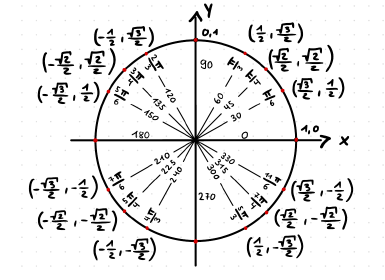
\includegraphics[width=\linewidth,keepaspectratio]{pictures/complex_numbers.png}
\end{figure}
\mysection[BurntOrange]{\centering Folgen und Reihen}
\mysubsection{Folgen}
\DEF{Folge}{Eine Folge (reeller Zahlen) ist eine Abbildung $a:\mathbb{N}^*\rightarrow\mathbb{R}$. Wir schreiben $a_n$ statt $a(n)$ und bezeichnen eine Folge mit $(a_n)_{n\geq 1}$.}

\LEM{2.1.3}{Sei $(a_n)_{n\geq 1}$. Dann gibt es höchstens ein $l\in\mathbb{R}$ mit der Eigenschaft: $\forall\varepsilon>0$ ist $\{n\in\mathbb{N}|a_n\not\in (l-\varepsilon,l+\varepsilon)\}$ endlich $\Leftrightarrow \forall\varepsilon>0$ ist $\{n\in\mathbb{N}|a_n\in(l-\varepsilon,l+\varepsilon)\}$ unendlich.}

\DEF{Konvergenz und Limes}{$(a_n)_{n\geq 1}$ heisst konvergent $\Leftrightarrow \exists l\in\mathbb{R}:\forall\varepsilon > 0$ ist $\{n\in\mathbb{N}|a_n\not\in (l-\varepsilon,l+\varepsilon)\}$ endlich. Nach Lemma 2.1.3 ist $l$ eindeutig bestimmt; sie wird mit $lim_{n\rightarrow +\infty}a_n$ bezeichnet und nennt sich Grenzwert oder Limes der Folge $(a_n)_{n\geq 1}$.}

\NOTE{2.1.5}{Jede konvergente Folge ist beschränkt.}

\LEM{2.1.6}{Sei $(a_n)_{n\geq 1}$. Folgende Aussagen sind äquivalent:

(1) $(a_n)_{n\geq 1}$ konvergiert gegen $l=lim_{n\rightarrow +\infty}a_n$.

(2) $\forall\varepsilon > 0,\exists N\geq 1: |a_n-l|<\varepsilon$ $\forall n\geq N$.}

\DEF{Divergenz}{$(a_n)_{n\geq 1}$ divergiert wenn...

(1) $(a_n)_{n\geq 1}$ konvergiert gegen $+\infty \Leftrightarrow$ $\forall l\in\mathbb{R},\exists N\in\mathbb{N}: a_n\geq l$ $\forall n\geq N$. Oder

(2) $(a_n)_{n\geq 1}$ konvergiert gegen $-\infty \Leftrightarrow$ $\forall l\in\mathbb{R},\exists N\in\mathbb{N}: a_n\leq l$ $\forall n\geq N$.
}

\SA{2.1.8 Rechenregeln für Limes}{Seien $(a_n)_{n\geq 1}$ und $(b_n)_{n\geq 1}$ mit $a=lim_{n\rightarrow\infty}a_n, b=lim_{n\rightarrow\infty}b_n$.
\begin{enumerate}
    \item $(a_n+b_n)_{n\geq 1}$ konvergiert und $lim_{n\rightarrow\infty}(a_n + b_n)=a+b$.
    \item $(a_n\cdot b_n)_{n\geq 1}$ konvergiert und $lim_{n\rightarrow\infty}(a_n \cdot b_n)=a\cdot b$.
    \item $\forall n\geq 1: b_n\not = 0$ und $b\not = 0 \Rightarrow (\frac{a_n}{b_n})_{n\geq 1}$ konvergiert und $lim_{n\rightarrow\infty}(\frac{a_n}{b_n})=\frac{a}{b}$.
    \item $\exists k\geq 1:a_n\leq b_n$ $\forall n\geq K \Rightarrow a \leq b$.
\end{enumerate}}

\DEF{Monotonie}{
(1) $(a_n)_{n\geq 1}$ ist monoton wachsend $\Leftrightarrow$ $\forall n\geq 1: a_n\leq a_{n+1}$.

(2) $(a_n)_{n\geq 1}$ ist monoton fallend $\Leftrightarrow$ $\forall n\geq 1: a_{n+1}\leq a_{n}$.}

\DEF{Sandwichlemma}{Seien $(a_n)_{n\geq 1},(b_n)_{n\geq 1},(c_n)_{n\geq 1}$ reelle Folgen s.d. $(a_n)_{n\geq 1},(b_n)_{n\geq 1}$ konvergieren mit $lim_{n\rightarrow\infty}a_n=lim_{n\rightarrow\infty}b_n$. $\exists N\in\mathbb{N}: a_n\leq c_n\leq b_n$ $\forall n\geq N \Leftrightarrow (c_n)_{n\geq 1}$ konvergiert und $lim_{n\rightarrow\infty}c_n=lim_{n\rightarrow\infty}a_n=lim_{n\rightarrow\infty}b_n$.}

\SA{2.2.2 Weierstrass}{(1) $(a_n)_{n\geq 1}$ monoton wachsend und nach oben beschränkt $\Rightarrow (a_n)_{n\geq 1}$ konvergiert mit $lim_{n\rightarrow\infty}a_n=sup\{a_n|n\geq 1\}$.

(2) $(a_n)_{n\geq 1}$ monoton fallend und nach unten beschränlt $\Rightarrow (a_n)_{n\geq 1}$ konvergiert mit $lim_{n\rightarrow\infty}a_n=inf\{a_n|n\geq 1\}$.}

\LEM{2.2.7 Bernoulli Ungleichung}{$(1+x)^n\geq 1+nx\ \forall n\in\mathbb{N},x>-1$.}

\DEF{Limes Inferior}{Sei $(a_n)_{n\geq 1}$ eine nach unten beschränkte folge. Sei $\forall n\geq 1:b_n=inf\{a_k|k\geq n\}$. Dann $\forall n\geq 1: b_n\leq b_{n+1}$ und $lim\ inf_{n\rightarrow\infty}a_n:=lim_{n\rightarrow\infty}b_n$.}

\DEF{Limes Superior}{Sei $(a_n)_{n\geq 1}$ eine nach oben beschränkte folge. Sei $\forall n\geq 1:c_n=sup\{a_k|k\geq n\}$. Dann $\forall n\geq 1: c_{n+1}\leq c_n$ und $lim\ sup_{n\rightarrow\infty}a_n:=lim_{n\rightarrow\infty}c_n$.}

\SA{}{Sei $(a_n)_{n\geq 1}$ eine beschränkte folge. Dann $lim\ inf_{n\rightarrow\infty}a_n\leq lim\ sup_{n\rightarrow\infty}a_n$.}

\SA{}{Sei $(a_n)_{n\geq 1}$ konvergente Folge reeller Zahlen mit $lim_{n\rightarrow\infty}a_n\geq 0$ und $(b_n)_{n\geq 1}$ eine nach oben beschränkte Folge reeller Zahlen. Dann $lim\ sup_{n\rightarrow\infty}a_nb_n=lim_{n\rightarrow\infty}a_n\cdot lim\ sup_{n\rightarrow\infty}b_n$.}

\SA{2.4.2 Cauchy Kriterium}{$(a_n)_{n\geq 1}$ konvergiert $\Leftrightarrow ((a_n)_{n\geq 1}$ ist beschränkt$)\ \land $ $(lim\ inf_{n\rightarrow\infty}a_n=lim\ sup_{n\rightarrow\infty}a_n)$(L2.4.1)

$\Leftrightarrow\ (a_n)_{n\geq 1}$ ist Cauchy-Folge $\Leftrightarrow\ \forall\varepsilon >0\ \exists N\geq 1: |a_n-a_m|<\varepsilon\ \forall n,m\geq N$.}

\DEF{Abgeschlossenes Intervall}{Eine Teilmenge $I\subseteq\mathbb{R}$ der Form:

(1) $a,b\in\mathbb{R},a\leq b: [a,b]$,

(2) $a\in\mathbb{R}: [a,+\infty)$,

(3) $a\in\mathbb{R}: (-\infty,a]$,

(4) $(-\infty,+\infty)=\mathbb{R}$.

Wir definieren die Länge $\mathcal{L}(I)$ als (1) $\mathcal{L}(I)=b-a$ und (2),(3),(4) $\mathcal{L}(I)=+\infty$.}

\NOTE{}{$I\subseteq\mathbb{R}$ ist beschränkte Teilmenge von $\mathbb{R} \Leftrightarrow$ $\mathcal{L}(I)<+\infty$.}

\NOTE{2.5.2}{$I\subseteq\mathbb{R}$ ist abgeschlossen $\Leftrightarrow\ \forall$ konvergente Folgen $(a_n)_{n\geq 1}, a_n\subseteq I$ gilt $lim_{n\rightarrow\infty}a_n\in I$.}

\NOTE{2.5.3}{Seien $I=[a,b],J=[c,d]$ mit $a\leq b, c\leq d,a,b,c,d\in\mathbb{R}$. Dann $I\subseteq J \Leftrightarrow c\leq a \land b\leq d \Rightarrow \mathcal{L}(I)=b-a\leq d-c = \mathcal{L}(J)$.}

\DEF{Monoton fallende Folge von Teilmengen}{Eine monoton fallende Folge von Teilmengen von $\mathbb{R}$ ist eine Folge $(X_n)_{n\geq 1},X_n\subseteq\mathbb{R}$ mit $X_1\supseteq X_2\supseteq ... \supseteq X_n \supseteq X_{n+1} \supseteq ...$ .}

\SA{2.5.5 Cauchy-Cantor (Intervallschachtelung)}{Sei $I_1\supseteq I_2\supseteq ... \supseteq I_n \supseteq I_{n+1} \supseteq ...$ eine Folge abgeschlossener Intervalle mit $\mathcal{L}(I_1)<+\infty$ und $\forall i\in\mathbb{N}: I_i\not = \emptyset$. Dann $\bigcap_{n\geq 1} I_n\not = \emptyset$. Falls zudem $lim_{n\rightarrow\infty}\mathcal{L}(I_n)=0$ gilt $|\bigcap_{n\leq 1}I_n|=1$.}


\DEF{Teilfolge}{Eine Teilfolge einer Folge $(a_n)_{n\geq 1}$ ist eine Folge $(b_n)_{n\geq 1}$ wobei $b_n=a_{l(n)}$ und $l:\mathbb{N}^*\rightarrow\mathbb{N}^*:l(n)<l(n+1)\ \forall n\geq 1$.}

\SA{2.5.9 Bolzano-Weierstrass}{Jede beschränkte Folge besitzt eine konvergente Teilfolge.}

\NOTE{2.5.10}{Sei $(a_n)_{n\geq 1}$ beschränkt. Dann gilt für jede konvergente Teilfolge $(b_n)_{n\geq 1}: lim\ inf_{n\rightarrow\infty}a_n\leq lim_{n\rightarrow\infty}b_n \leq lim\ sup_{n\rightarrow\infty}a_n$.}

\mysubsection{Folgen in $\mathbb{R}^d$ und $\mathbb{C}$}
Eine Folge in $\mathbb{R}^d$ ist eine Abbildung $a:\mathbb{N}^*\rightarrow\mathbb{R}^d$. Wir schreiben $a_n$ statt $a_n$ und bezeichnen die Folge mit $(a_n)_{n\geq 1}$.

\DEF{Konvergenz}{Sei $||\cdot||$ die euklidische Norm auf $\mathbb{R}^d$. $(a_n)_{n\geq 1}\in\mathbb{R}^d$ ist konvergent $\Leftrightarrow\ \exists a\in\mathbb{R}^d:\forall\varepsilon > 0\ \exists N\geq 1: ||a_n-a||<\varepsilon\ \forall n\geq \mathbb{N}$. Falls solch ein $a$ existiert, ist es eindeutig bestimmt durch $lim_{n\rightarrow\infty}a_n=a$.}

\SA{2.6.3}{Sei $a_n=(a_{n,1},...,a_{n,d})$ die Koordinaten von $a_n$. Sei $b=(b_1,...,b_d)$. Folgende Aussagen sind äquivalent:

(1) $lim_{n\rightarrow\infty}a_n=b$

(2) $lim_{n\rightarrow\infty}a_{n,j}=b_j\ \forall 1\leq j \leq d$.}

\DEF{Häufungspunkt}{Sei $(a_n)_{n\geq 1}$. $c\in\mathbb{R}$ ist Häufungspunkt von $(a_n)_{n\geq 1} \Leftrightarrow \exists$ Teilfolge von $(a_n)_{n\geq 1}$, die gegen $c$ konvergiert. Beispiele:

(1) $a_n=(-1)^n+\frac{1}{n}$. Häufungspunkte sind: $\pm 1$.

(2) $a:\mathbb{N}^*\rightarrow [0,1]\cap\mathbb{Q}$ surjektiv hat beliebig viele Häufungspunkte, weil jede rationale Zahl w.z.B. $\frac{1}{4}=\frac{2}{8}=\frac{3}{12}=...$ kommt unendlich oft vor in $(a_n)_{n\geq 1}$.}

\SA{2.6.6}{(1) $(a_n)_{n\geq 1}$ konvergiert $\Leftrightarrow$ $(a_n)_{n\geq 1}$ ist eine Cauchy-Folge $\Leftrightarrow\ \forall\varepsilon > 0\ \exists N\geq 1: ||a_n-a_m|| < \varepsilon\ \forall n,m\geq N$.

(2) Jede beschränkte Folge hat eine konvergente Teilfolge.}

\mysubsection{Reihen}
\DEF{Reihe}{Sei $(a_n)_{n\geq 1}$ eine Folge in $\mathbb{R}$ oder $\mathbb{C}$. Dann ist $\sum_{k=1}^{\infty}a_k$ eine Reihe.}

\DEF{Folge der Partialsummen}{Sei $(a_n)_{n\geq 1}$. Dann ist die Folge der Partialsummen definiert als $S_n=\sum_{k=1}^{n}a_k$.}

\DEF{Konvergenz}{Die Reihe $\sum_{k=1}^{\infty}a_k$ ist konverget, falls die Folge $(S_n)_{n\geq 1}$ der Partialsummen konvergiert. Dann $\sum_{k=1}^{\infty}a_k:=lim_{n\rightarrow\infty}S_n$.}

\SA{2.7.4}{Seien $\sum_{n=1}^\infty a_k, \sum_{n=1}^\infty b_k$ konvergent, sowie $\alpha \in\mathbb{C}$. 

(1) Dann ist $\sum_{n=1}^\infty (a_k + b_k)$ konvergent und $\sum_{n=1}^\infty (a_k + b_k)=(\sum_{n=1}^\infty a_k)+(\sum_{n=1}^\infty b_k)$.

(2) Dann ist $\sum_{k=1}^\infty \alpha\cdot a_k$ konvergent und $\sum_{n=1}^\infty \alpha\cdot a_k = \alpha\cdot\sum_{n=1}^\infty a_k$.}

\SA{2.7.5 Cauchy Kriterium}{Die Reihe $\sum_{k=1}^\infty a_k$ ist konvergent $\Leftrightarrow\ \forall\varepsilon > 0,\exists N\geq 1: |\sum_{k=n}^ma_k|<\varepsilon\ \forall m\geq n \geq N$.}

\SA{2.7.6}{Sei $\sum_{k=1}^\infty$ eine Reihe mit $a_k\geq 0\ \forall k\in\mathbb{N}^*$. $\sum_{k=1}^\infty a_k$ konvergiert $\Leftrightarrow (S_n)_{n\geq 1},S_n=\sum_{k=1}^na_k$ ist nach oben beschränkt.}

\COR{2.7.7 Vergleichssatz}{Seien $\sum_{k=1}^\infty a_k, \sum_{k=1}^\infty b_k$ mit $0\leq a_k \leq b_k\ \forall k\geq 1$. Dann 

(1) $\sum_{k=1}^\infty b_k$ konvergent $\Rightarrow \sum_{k=1}^\infty a_k$ konvergent. 

(2) $\sum_{k=1}^\infty a_k$ divergent $\Rightarrow \sum_{k=1}^\infty b_k$ divergent.}

\DEF{Absolute Konvergenz}{$\sum_{k=1}^{\infty}a_k$ ist absolut konvergent $\Leftrightarrow \sum_{k=1}^{\infty}|a_k|$ konvergiert.}

\DEF{Bedingte Konvergenz}{$\sum_{k=1}^{\infty}a_k$ ist bedingt konvergent $\Leftrightarrow \sum_{k=1}^{\infty}a_k$ ist konvergent aber nicht absolut konvergent.}

\SA{2.7.10}{Eine absolut konvergente Reihe $\sum_{k=1}^{\infty}a_k$ ist auch konvergent und es gilt: $|\sum_{k=1}^{\infty}a_k|\leq\sum_{k=1}^{\infty}|a_k|$. Umgekehrt gilt dies jedoch nicht. Beispiel: $\sum_{k=1}^{\infty}(-1)^{k+1}\frac{1}{k}=1-\frac{1}{2}+\frac{1}{3}-\frac{1}{4}+...$ konvergiert, ist aber nicht absolut konvergent.}

\SA{2.7.12 Leibniz}{Sei $(a_n)_{n\geq 1}$ monoton fallend mit $a_n\geq 0\ \forall n\geq 1,lim_{n\rightarrow\infty}a_n=0$. Dann konvergiert $S:=\sum_{k=1}^{\infty}(-1)^{k+1}a_k$ und es gilt $a_1-a_2\leq S \leq a_1$.}

\DEF{Umordnung}{Eine Reihe $\sum_{n=1}^{\infty}a_n'$ ist eine Umordnung von $\sum_{n=1}^{\infty}a_n \Leftrightarrow\ \exists $ Bijektion $\phi:\mathbb{N}^*\rightarrow\mathbb{N}^*:a_n'=a_{\phi(n)}$. Umordnungen von bedingt konvergenten Reihen können andere Werte haben als die Ausgangsreihe.}

\NOTE{2.7.15}{Aus Riemann folgt, dass es überabzählbar viele Bijektionen von $\mathbb{N}^*$ gibt.}

\SA{2.7.16 Dirichlet 1837}{$\sum_{n=1}^{\infty}a_n$ konvergiert absult $\Rightarrow$ jede Umordnung der Reihe konvergiert und hat den selben Grenzwert.}

\SA{2.7.17 Quotientenkriterium}{Sei $(a_n)_{n\geq 1}$ mit $a_n\not = 0\ \forall n\geq 1$.

(1) $lim\ sup_{n\rightarrow\infty}\frac{|a_{n+1}|}{|a_n|}<1 \Rightarrow \sum_{n=1}^{\infty}a_n$ konvergiert absolut.

(2) $lim\ inf_{n\rightarrow\infty}\frac{|a_{n+1}|}{|a_n|}>1 \Rightarrow \sum_{n=1}^{\infty}a_n$ divergiert.

(2)* $\exists N\in\mathbb{N}:\forall n\geq N:\frac{|a_{n+1}|}{|a_n|}\geq 1\Rightarrow \sum_{n=1}^{\infty}a_n$ divergiert.}

\SA{2.7.20 Wurzelkriterium}{Sei $(a_n)_{n\geq 1}$.

(1) $lim\ sup_{n\rightarrow\infty}\sqrt[n]{|a_n|}<1 \Rightarrow \sum_{n=1}^{\infty}a_n$ konvergiert absolut.

(2) $lim\ sup_{n\rightarrow\infty}\sqrt[n]{|a_n|}>1 \Rightarrow \sum_{n=1}^{\infty}a_n$ und $\sum_{n=1}^{\infty}|a_n|$ divergieren.}

\DEF{Geometrische Reihe}{Sei $q\in\mathbb{C},|q|<1$. Dann $\sum_{k=0}^{\infty}q^k=\frac{1}{1-q}$.}

\DEF{Harmonische Reihe}{Die Reihe $\sum_{n=1}^\infty\frac{1}{n}$ divergiert.}

\DEF{Exponentialreihe}{Die Reihe $exp(z):=\sum_{n=0}^{\infty}\frac{z^n}{n!}=1+z+\frac{z^2}{2!}+\frac{z^3}{3!}+...$ konvergiert absolut.}

\DEF{Potenzreihe}{Sei $(c_n)_{n\geq 0}$ in $\mathbb{R}$ oder $\mathbb{C}$. Falls $lim\ sup_{n\rightarrow\infty}\sqrt[n]{|c_n|}$ existiert, definieren wir $\rho=\begin{cases}
    +\infty & \text{if $lim\ sup_{n\rightarrow\infty}\sqrt[n]{|c_n|}=0$}\\
    \frac{1}{lim\ sup_{n\rightarrow\infty}\sqrt[n]{|c_n|}} & \text{if $lim\ sup_{n\rightarrow\infty}\sqrt[n]{|c_n|}>0$}
\end{cases}$

Die Potenzreihe $\sum_{n=0}^{\infty}c_nz^k$ konvergiert absolut $\forall\ |z|<\rho$ und divergiert $\forall\ |z|>\rho$. Auf dem Konvergenzradius $|z|=\rho$ kann alles passieren.}

\DEF{Zeta Funktion}{Sei $s>1$ und $\zeta(s)=\sum_{n=1}^{\infty}\frac{1}{n^s}$. $\zeta(s)$ konvergiert.}

\mysubsection{Doppelfolgen und Doppelreihen}
Gegeben eine Doppelfolge $(a_{ij})_{i,j\geq 0}$. Dann können $\sum_{i=0}^{\infty}(\sum_{j=0}^{\infty}a_{ij})=S_0+S_1+S_2+...$ und $\sum_{j=0}^{\infty}(\sum_{i=0}^{\infty}a_{ij})=b_0+b_1+b_2+...$ beide konvergent sein mit verschiedenen Grenzwerten. Wir nennen $\sum_{i,j\geq 0}a_{ij}$ eine Doppelreihe.

\DEF{Lineare Anordnung}{$\sum_{k=0}^{\infty}b_k$ ist eine lineare Anordnung der Doppelreihe $\sum_{i,j\geq 0}a_{ij} \Leftrightarrow\ \exists$ Bijektion $\sigma:\mathbb{N}\rightarrow\mathbb{N}\times\mathbb{N}:b_k=a_{\sigma(k)}$.}

\DEF{Cauchy 1821 (Doppelreihensatz)}{Angenommen $\exists\ B\geq 0:\sum_{i=0}^m\sum_{j=0}^m|a_{ij}|\leq B\ \forall m\geq 0$. Dann konvergieren die folgenden Reihen absolut:
$S_i:=\sum_{j=0}^{\infty}a_{ij}\ \forall i\geq 0$ und $U_j:=\sum_{i=0}^{\infty}a_{ij}\ \forall j\geq 0$ sowie $\sum_{i=0}^{\infty}S_i$ und $\sum_{j=0}^{\infty}U_i$ und es gilt: $\sum_{i=0}^{\infty}S_i=\sum_{j=0}^{\infty}U_j$. 

Zudem konvergiert jede lineare Anordnung der Doppelreihe absolut, mit selbem Grenzwert.}

\DEF{Cauchy Produkt}{Das Cauchy Produkt der Reihen $\sum_{i=0}^{\infty}a_i,\sum_{j=0}^{\infty}b_j$ ist die Reihe $\sum_{n=0}^{\infty}(\sum_{j=0}^na_{n-j}b_j)=a_0b_0+(a_0b_1+a_1b_0)+(a_0b_2+a_1b_1+a_2b_0)+...$}

\SA{2.7.26}{Die Reihen $\sum_{i=0}^{\infty}a_i,\sum_{j=0}^{\infty}b_j$ konvergieren absolut $\Leftrightarrow$ ihr Cauchy Produkt konvergiert und es gilt: $\sum_{n=0}^{\infty}(\sum_{j=0}^na_{n-j}b_j)=(\sum_{i=0}^{\infty}a_i)(\sum_{j=0}^{\infty}b_j)$.}

\SA{2.7.28}{Sei $f_n:\mathbb{N}\rightarrow\mathbb{R}$ eine Folge. Wir nehmen an, dass:

(1) $\forall j\in\mathbb{N},\exists\ f(j):=lim_{n\rightarrow\infty}f_n(j)$

(2) $\exists g:\mathbb{N}\rightarrow [0,\infty)$ s.d.
\begin{enumerate}
    \item[2.1] $|f_n(j)|\leq g(j)\ \forall j\geq 0,\ \forall n\geq 0$.
    \item[2.2] $\sum_{j=0}^{\infty}g(j)$ konvergiert.
\end{enumerate}

Dann $\sum_{j=0}^{\infty}f(j)=lim_{n\rightarrow\infty}\sum_{j=0}^{\infty}f_n(j)$.
}

\COR{2.7.29}{$\forall z\in\mathbb{C}$ konvergiert die Folge $((1+\frac{z}{n})^n)_{n\geq 1}$ und $lim_{n\rightarrow\infty}(1+\frac{z}{n})^n=exp(z)$.}




\mysection[WildStrawberry]{\centering Stetige Funktionen}
\mysubsection{Reellwertige Funktionen}
Sei $D$ eine beliebige Menge. Die Menge $R^D$ aller Funktionen $f:D\rightarrow \mathbb{R}$ bildet einen Vektorraum über $\mathbb{R}$, wobei Addition, skalare Multiplikation, und das Produkt gegeben sind durch: 
\begin{enumerate}
    \item $(f_1+f_2)(x)=f_1(x)+f_2(x)$
    \item $(\alpha \cdot f)(x)=\alpha \cdot f(x)$
    \item $(f_1\cdot f_2)(x)=f_1(x)f_2(x)$
\end{enumerate}
wobei $f_1,f_2,f\in\mathbb{R}^D,x\in D,\alpha\in\mathbb{R}$.

Eine konstante Funktion ist eine, die immer denselben Wert annimt. Darunter gibt es die Funktionen $\mathtt{0},\mathtt{1}\in\mathbb{R}^D$:
\begin{enumerate}
    \item $\mathtt{0}(x)=0\ \forall x\in D$
    \item $\mathtt{1}(x)=1\ \forall x\in D$
\end{enumerate}
Offensichtlich gilt $f+\mathtt{0}=f,g\cdot\mathtt{1}=g\ \forall f,g\in\mathbb{R}^D$. $\mathbb{R}^D$ versehen mit $+,\cdot$ erfüllt die Körperaxiome (ausser: falls $|D|\geq 2$ gibt es immer ein $f\not = \mathtt{0}$, das kein multiplikatives Inverses besitzt.

Auf $\mathbb{R}^D$ definieren wir eine Ordnung: $f\leq g \Leftrightarrow f(x)\leq g(x)\ \forall x\in D$. Weiter gilt $f$ ist nicht negativ $\Leftrightarrow \mathtt{0}\leq f$.

\DEF{Beschränktheit}{Sei $f\in\mathbb{R}^D$. Dann $f(D)=\{f(x)|x\in D\}$ und 
\begin{enumerate}
    \item $f$ ist nach oben beschränkt $\Leftrightarrow f(D)\subseteq\mathbb{R}$ ist nach oben beschränkt.
    \item $f$ ist nach unten beschränkt $\Leftrightarrow f(D)\subseteq\mathbb{R}$ ist nach unten beschränkt.
    \item $f$ ist beschränkt $\Leftrightarrow f(D)\subseteq\mathbb{R}$ ist beschränkt.
\end{enumerate}}

\DEF{Monotonie}{Sei $D\subseteq\mathbb{R}$. Eine Funktion $f:D\rightarrow\mathbb{R}$ ist
\begin{enumerate}
    \item monoton wachsend $\Leftrightarrow\ \forall x,y\in D: x\leq y \Rightarrow f(x)\leq f(y)$.
    \item streng monoton wachsend $\Leftrightarrow\ \forall x,y\in D: x<y\Rightarrow f(x)<f(y)$.
    \item monoton fallend $\Leftrightarrow\ \forall x,y\in D: x\leq y\Rightarrow f(x)\geq f(y)$.
    \item streng monoton fallend $\Leftrightarrow\ \forall x,y\in D: x<y\Rightarrow f(x)>f(y)$
    \item monoton $\Leftrightarrow (f$ ist monoton wachsend$) \lor (f$ ist monoton fallend$)$.
    \item streng monoton $\Leftrightarrow (f$ ist streng monoton wachsend$) \lor (f$ ist streng monoton fallend$)$.
\end{enumerate}}

\NOTE{3.1.3}{Sei $n\in\mathbb{N}$. Sei $f:\mathbb{R}\rightarrow\mathbb{R}$ definiert durch $x\mapsto x^n$. Dann $f$ (streng) monoton wachsend $\Leftrightarrow n\ mod\ 2 = 1$.}

\SA{}{Sei $f:[0,1]\rightarrow[0,\infty)$ monoton. Dann ist das Bild von $f$ immer ein beschränktes Intervall $[a,b]\subset[0,\infty)$ mit $0\leq a\leq b < \infty \Rightarrow f$ nicht surjektiv.}


\mysubsection{Stetigkeit}
\DEF{Stetigkeit in einem Punkt}{Sei $D\subseteq\mathbb{R},x_0\in D$. $f:D\rightarrow\mathbb{R}$ ist in $x_0$ stetig $\Leftrightarrow\ \forall\varepsilon > 0\ \exists\delta > 0:\forall x\in D\ (|x-x_0|<\delta\Rightarrow |f(x)-f(x_0)| < \varepsilon)$.}
\begin{figure}[H]
 \centering
 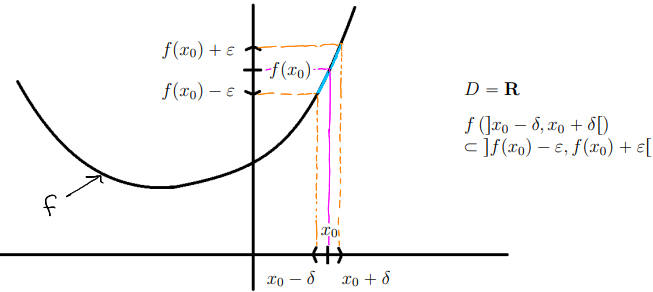
\includegraphics[width=\linewidth,keepaspectratio]{pictures/stetigkeit_in_einem_punkt.png} 
\end{figure}

\DEF{Stetigkeit einer Funktion}{$f:D\rightarrow\mathbb{R}$ ist stetig $\Leftrightarrow f$ ist in jedem Punkt $x\in D$ stetig.}

\SA{3.2.4 Folgenstetigkeit}{Sei $x_0\in D\subseteq\mathbb{R}$ und $f:D\rightarrow\mathbb{R}$ stetig in $x_0$ $\Leftrightarrow\ \forall (a_n)_{n\geq 1}\subseteq D: lim_{n\rightarrow\infty}a_n=x_0\Rightarrow lim_{n\rightarrow\infty}f(a_n)=f(x_0)$.}

\COR{3.2.5}{Sei $x_0\in D\subseteq\mathbb{R},\lambda\in\mathbb{R}$ und $f:D\rightarrow\mathbb{R},g:D\rightarrow\mathbb{R}$ beide stetig in $x_0$.

(1) Dann sind $f+g,\lambda\cdot f,f\cdot g$ stetig in $x_0$.

(2) Falls $g(x_0)\not = 0$ dann ist $\frac{f}{g}:D\cap\{x\in D:g(x)\not =0\}\rightarrow\mathbb{R}$ definiert durch $x\mapsto\frac{f(x)}{g(x)}$ stetig in $x_0$.}

\DEF{Polynomiale Funktion}{Eine polynomiale Funktion $P:\mathbb{R}\rightarrow\mathbb{R}$ ist eine Funktion der Form $P(x)=a_nx^n+...+a_0$ wobei $a_n,...,a_0\in\mathbb{R}$. Falls $a_n\not = 0$ ist $n$ der Grad von $P$.}

\COR{3.2.7}{Polynomiale Funktionen sind auf ganz $\mathbb{R}$ stetig.}

\COR{3.2.8}{Seien $P,Q$ polynomiale Funktionen auf $\mathbb{R}$ mit $Q\not =\mathtt{0}$. Seien $x_1,...,x_m$ die Nullstellen von $Q$. Dann ist $\frac{P}{Q}:\mathbb{R}\ \{x_1,...,x_m\}\rightarrow\mathbb{R}$ definiert duch $x\mapsto\frac{P(x)}{Q(x)}$ stetig.}

\mysubsection{Zwischenwertsatz}
Seien $x_1,x_2\in\mathbb{R}$. Dann liegt $c$ zwischen $x_1$ und $x_2 \Leftrightarrow (x_1\leq x_2 \land c\in[x_1,x_2]) \lor (x_2\leq x_1 \land c\in[x_2,x_1])$.

\SA{3.3.1 Bolzano 1817}{Sei $I\subseteq\mathbb{R}$ ein Intervall, $f:I\rightarrow\mathbb{R}$ eine stetige Funktion und $a,b\in I$. Dann $\forall c$ zwischen $f(a)$ und $f(b)$ gibt es ein $z$ zwischen $a$ und $b$ mit $f(z)=c$.}
\begin{figure}[H]
 \centering
 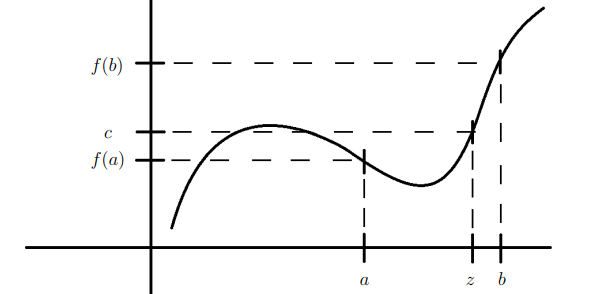
\includegraphics[width=\linewidth,keepaspectratio]{pictures/zwischenwertsatz.png} 
\end{figure}

\COR{3.3.2}{Sei $P(x)=a_nx^n+a_{n-1}x^{n-1}+...+a_0$ ein Polynom mit $a_n\not = 0$ und $n$ ungerade. Dann besitzt $P$ mindestens eine Nullstelle in $\mathbb{R}$.}

\mysubsection{Min-Max Satz}
\DEF{Kompakt}{Ein Intervall $I\subseteq\mathbb{R}$ ist kompakt, falls es von der Form $I=[a,b], a\leq b$ ist.}

\DEF{Notation}{Sei $D$ eine Menge und $f,g:D\rightarrow\mathbb{R}$.
\begin{itemize}
    \item $\forall x\in D: |f|(x):=|f(x)|$
    \item $\forall x\in D: max(f,g)(x):=max(f(x),g(x))$
    \item $\forall x\in D: min(f,g)(x):=min(f(x),g(x))$
\end{itemize}}

\LEM{3.4.3}{Sei $D\subseteq\mathbb{R},x_0\in D$ und $f,g:D\rightarrow\mathbb{R}$ stetig in $x_0$. Dann sind $|f|,max(f,g),min(f,g)$ stetig in $x_0$.}

\LEM{3.4.4}{Sei $(x_n)_{n\geq 1}$ eine konvergente Folge in $\mathbb{R}$ mit $lim_{n\rightarrow\infty}X_n\in\mathbb{R}$. Sei $a\leq b$. Falls $\{x_n:n\geq 1\}\subseteq[a,b] \Rightarrow lim_{n\rightarrow\infty}x_n\in[a,b]$.}

\SA{3.4.5}{Sei $I=[a,b]$. Sei $f:I\rightarrow\mathbb{R}$ stetig. Dann $\exists u,v\in I: f(u)\leq f(x)\leq f(v)\ \forall x\in I \Leftrightarrow f$ ist beschränkt.}

\mysubsection{Satz der Umkehrabbildung}
\SA{3.5.1}{Seien $D_1,D_2\subseteq\mathbb{R}$, $f:D_1\rightarrow D_2,$ $g:D_2\rightarrow\mathbb{R},$ $x_0\in D_1$. Dann $f$ in $x_0$ und $g$ in $f(x_0)$ stetig $\Leftrightarrow g\circ f:D_1\rightarrow\mathbb{R}$ in $x_0$ stetig. }

\COR{3.5.2}{Falls $f$ auf $D_1$ und $g$ auf $D_2$ stetig $\Rightarrow g\circ f$ auf $D_1$ stetig.}

\SA{3.5.3}{Sei $I\subseteq\mathbb{R}$ ein Intervall und $f:I\rightarrow\mathbb{R}$ stetig, streng monoton. Dann ist $J:=f(i)\subseteq\mathbb{R}$ ein Intervall und $f^{-1}:J\rightarrow I$ ist stetig, streng monoton.}

\mysubsection{Reelle Exponentialfunktion}
\SA{3.6.1}{$exp:\mathbb{R}\rightarrow(0,\infty)$ ist stetig, streng monoton wachsend, und surjektiv.}

\DEF{Natürlicher Logarithmus}{Die Umkehrabbildung von $exp:\mathbb{R}\rightarrow(0,\infty)$ ist der natürliche Logarithmus $ln:(0,\infty)\rightarrow\mathbb{R}$.}

\COR{3.6.5}{$ln:(0,\infty)\rightarrow\mathbb{R}$ ist stetig, streng monoton wachsend, und bijektiv.}

\COR{3.6.6}{
\begin{enumerate}
    \item Für $a>0$ ist $(0,\infty)\rightarrow(0, \infty), x\mapsto x^a$ stetig, streng monoton wachsend, und bijektiv.
    \item Für $a < 0$ ist $(0,\infty)\rightarrow(0, \infty), x\mapsto x^a$ stetig, streng monoton fallend, und bijektiv.
\end{enumerate}}

\mysubsection{Konvergenz von Funktionenfolgen}
Sei $D$ eine Menge. Eine (reellwertige) Funktionenfolge ist eine Abbildung $\mathbb{N}\rightarrow\mathbb{R}^D,n\mapsto f_n$. D.h. jedes $f_n$ ist eine Funktion $D\rightarrow\mathbb{R}$.

Für eine Funktionenfolge schreiben wir $(f_n)_{n\geq 0}$. $\forall x\in D$ erhalten wir eine Folge $(f_n(x))_{n\geq 0}$ in $\mathbb{R}$.

\DEF{Punktweise Konvergenz}{Die Funktionenfolge $(f_n)_{n\geq 0}$ konvergiert punktweise gegen $f:D\rightarrow\mathbb{R}$, falls $\forall x\in D:lim_{n\rightarrow\infty}f_n(x)=f(x)$ $\Leftrightarrow$ $\forall x\in D\ \forall\varepsilon > 0\ \exists N\in\mathbb{N}\ \forall n\geq N: |f_n(x)-f(x)|<\varepsilon$. $f$ ist nicht zwingend in $D$ stetig.}

\DEF{Gleichmässige Konvergenz}{Die Funktionenfolge $f_n:D\rightarrow\mathbb{R}$ konvergiert gleichmässig in $D$ gegen $f:D\rightarrow\mathbb{R}$, falls $\forall\epsilon > 0$ $\exists N\in\mathbb{N}$ s.d. $\forall n\geq N,\forall x\in D: |f_n(x)-f(x)|<\epsilon$ $\Leftrightarrow f_n$ liegt komplett im $\epsilon$-Schlauch um $f$.}

\SA{3.7.4}{Sei $D\subseteq\mathbb{R}$ und $f_n:D\rightarrow\mathbb{R}$ eine Funktionenfolge bestehend aus (in $D$) stetigen Funktionen die (in $D$) gleichmässig gegen $f:D\rightarrow\mathbb{R}$ konvergieren. Falls $f_n$ $\forall n\geq 1$ stetig in $x_0\in D \Rightarrow f$ stetig in $x_0$.}

\COR{3.7.6 Cauchy Kriterium}{Die Funktionenfolge $f_n:D\rightarrow\mathbb{R}$ konvergiert gleichmässig in $D$ $\Leftrightarrow$ $\forall\varepsilon > 0\ \exists N\geq 1:$ $\forall n,m\geq N\ \forall x\in D:$ $ |f_n(x)-f_m(x)|<\varepsilon$.}

\COR{3.7.7}{Sei $D\subseteq\mathbb{R}$. Falls $f_n:D\rightarrow\mathbb{R}$ gleichmässig konvergente Folge stetiger Funktionen $\Rightarrow f(x):=lim_{n\rightarrow\infty}f_n(x)$ stetig.}

\mysubsection{Reihen von Funktionen}
\DEF{Konvergenz}{Die Reihe $\sum_{k=0}^{\infty}f_k(x)$ konvergiert punktweise (resp. gleichmässig) in $D$, falls die Funktionenfolge $S_n(x):=\sum_{k=0}^nf_k(x)$ punktweise (resp. gleichmässig) konvergiert.}

\SA{3.7.9}{Sei $D\subseteq\mathbb{R}$ und $f_n:D\rightarrow\mathbb{R}$ eine Funktionenfolge. Sei $|f_n(x)|\leq c_n\in[0,\infty)\ \forall x\in D$ und $\sum_{n=0}^{\infty}c_n$ konvergent. Dann konvergiert $\sum_{n=0}^{\infty}f_n(x)$ gleichmässig in $D$. Falls alle $f_n$ in $D$ stetig sind, dann ist $f(x):=\sum_{n=0}^{\infty}f_n(x)$ eine in $D$ stetige Funktion.}

\SA{3.7.11}{Sei $\sum_{k=0}^{\infty}c_kx^k$ eine Potenzreihe mit $\rho > 0$. Sei $f(x):=\sum_{k=0}^{\infty}c_kx^k,\ |x|<\rho$. Dann gilt $\forall 0\leq r < \rho$ konvergiert $\sum_{k=0}^{\infty}c_kx^k$ gleichmässig auf $[-r,r]$ und $f:(-\rho,\rho)\rightarrow\mathbb{R}$ stetig.}


\mysubsection{Trigonometrische Funktionen}
\DEF{Sinus}{Sei $z\in\mathbb{C}$. $sin(z) = z-\frac{z^3}{3!}+\frac{z^5}{5!}-\frac{z^7}{7!}+...=\sum_{n=0}^{\infty}\frac{(-1)^nz^{2n+1}}{(2n+1)!}$.}

\DEF{Cosinus}{Sei $z\in\mathbb{C}$. $cos(z) = 1-\frac{z^2}{2!}+\frac{z^4}{4!}-\frac{z^6}{6!}+...=\sum_{n=0}^{\infty}\frac{(-1)^nz^{2n}}{(2n)!}$.}

\DEF{Tangens}{$tan(z)=\frac{sin(z)}{cos(z)}, z\not\in\frac{\pi}{2}+\pi\cdot\mathbb{Z}$.}

\DEF{Cotangens}{$cot(z)=\frac{cos(z)}{sin(z)}, z\not\in\pi\cdot\mathbb{Z}$.}

\DEF{Arcsin}{$arcsin:[-1,1]\rightarrow[-\frac{\pi}{2},\frac{\pi}{2}]$ ist die Umkehrfunktion von $sin:[-\frac{\pi}{2},\frac{\pi}{2}]\rightarrow[-1,1]$. Also $arcsin:=sin^{-1}$.}

\DEF{Arccos}{$arccos:[-1,1]\rightarrow[0,\pi]$ ist die Umkehrfunktion von $cos:[0,\pi]\rightarrow[-1,1]$. Also $arccos:=cos^{1}$.}

\DEF{Arctan}{$arctan:(-\infty, \infty)\rightarrow (-\frac{\pi}{2},\frac{\pi}{2})$ ist die Umkehrfunktion von $tan:(-\frac{\pi}{2},\frac{\pi}{2})\rightarrow(-\infty, \infty)$. Also $arctan:=tan^{-1}$. $arctan(0)=0, arctan(1)=\frac{\pi}{4}$, $\lim_{x\rightarrow\infty}arctan(x)=\frac{\pi}{2}$, $\lim_{x\rightarrow-\infty}arctan(x)=\frac{-\pi}{2}$.}

\DEF{Arccot}{$arccot:(-\infty, \infty)\rightarrow (0,\pi)$ ist die Umkehrfunktion von $cot:(0,\pi)\rightarrow(-\infty,\infty)$. Also $arccot:=cot^{-1}$.}

\NOTE{}{Für $x\in\mathbb{R}$ ist $cos(x)=Re(exp(ix))$, $sin(x)=Im(exp(ix))$.}

\NOTE{}{Die Reihen $sin(z)$ und $cos(z)$ konvergieren absolut $\forall z\in\mathbb{C}$. Konvergenzradius ist also in beiden Fällen $\infty$.}

\SA{3.8.1}{$sin:\mathbb{R}\rightarrow\mathbb{R}$ und $cos:\mathbb{R}\rightarrow\mathbb{R}$ sind stetig.}

\SA{3.8.2}{
\begin{enumerate}
    \item $exp(iz)=cos(z)+isin(z)\ \forall z\in\mathbb{C}$
    \item $cos(z)=cos(-z)$ und $sin(-z)=-sin(z)\ \forall z\in\mathbb{C}$
    \item $sin(z)=\frac{e^{iz}-e^{-iz}}{2i}$,\  $cos(z)=\frac{e^{iz}+e^{-iz}}{2}$
    \item $sin(z+w)=sin(z)cos(w)+cos(z)sin(w)$\\ $cos(z+w)=cos(z)cos(w)-sin(z)sin(w)$
    \item $cos(z)^2+sin(z)^2=1\ \forall z\in\mathbb{C}$
    \item $sin(z) - sin(w) = 2sin(\frac{z-w}{2})cos(\frac{z+w}{2})$ $cos(z)-cos(w)=-2sin(\frac{z-w}{2})sin(\frac{z+w}{2})$
\end{enumerate}}

\COR{3.8.3 (Winkelverdopplungsformeln)}{
\begin{enumerate}
    \item $sin(2z)=2sin(z)cos(z)$
    \item $cos(2z)=cos(z)^2-sin(z)^2$
    \item $cos(2z)=1-2sin(z)^2\Leftrightarrow sin(z)^2=\frac{1}{2}-\frac{cos(2z)}{2}$.
    \item $cos(z)^2=\frac{cos(2z)}{2}+\frac{1}{2}$.
\end{enumerate}}

\mysubsection{Die Kreiszahl $\pi$}
\SA{3.9.1}{$sin(x)$ hat auf $(0,\infty)$ mindestens eine Nullstelle. Sei $\pi=inf\{t:t>0,sin(t)=0\}$ die erste Nullstelle. Dann gilt:
\begin{enumerate}
    \item $sin(\pi)=0$, $\pi\in(2,4)$.
    \item $\forall x\in (0,\pi):sin(x)>0$.
    \item $e^{\frac{i\pi}{2}}=i$.
\end{enumerate}}

\COR{3.9.2}{$x\geq sin(x) \geq x-\frac{x^3}{3!}\ \forall 0 \leq x \leq \sqrt{6}$.}

\COR{3.9.3}{
\begin{enumerate}
    \item $e^{i\pi}=-1,\ e^{i2\pi}=1$
    \item $sin(x+\frac{\pi}{2})=cos(x),cos(x+\frac{\pi}{2})=-sin(x)\ \forall x\in\mathbb{R}.$
    \item $sin(x+\pi)=-sin(x), sin(x+2\pi)=sin(x)\ \forall x\in\mathbb{R}$.
    \item $cos(x+\pi)=-cos(x), cos(x+2\pi)=cos(x)\ \forall x\in\mathbb{R}$.
    \item $\{x:sin(x)=0\}=\{k\cdot\pi:k\in\mathbb{Z}\}$.\\
            $sin(x)>0\ \forall x\in(2k\pi,(2k+1)\pi),\  k\in\mathbb{Z}$.\\
            $sin(x)<0\ \forall x\in((2k+1)\pi, (2k+2)\pi),\  k\in\mathbb{Z}$.
    \item $\{x:cos(x)=0\}=\{k\cdot\pi+\frac{\pi}{2}:k\in\mathbb{Z}\}$.\\
            $cos(x)>0\ \forall x\in(2k\pi-\frac{\pi}{2},(2k+1)\pi-\frac{\pi}{2}),\  k\in\mathbb{Z}$.\\
            $cos(x)<0\ \forall x\in((2k+1)\pi-\frac{\pi}{2}, (2k+2)\pi-\frac{\pi}{2}),\  k\in\mathbb{Z}$.
\end{enumerate}}

\DEF{Komplexer Einheitskreis}{Sei $S^1=\{z\in\mathbb{C}:|z|=1\}$ der komplexe Einheitskreis. Dann $cis:[0,2\pi)\rightarrow S^1,x\mapsto e^{ix}$ bijektiv.}

\DEF{Bogenmass}{Sei $x\in\mathbb{R},n\in\mathbb{N}^*,z_{n,k}:=e^{\frac{ikx}{n}}\in S^1$ für $0\leq k\leq n$. Dann ist $L_n:=\sum_{k=1}^n|z_{n,k}-z_{n,k-1}|=n|z_{n,1}-z_{n,0}|=n\cdot 2|sin(\frac{x}{2n})|$ die Länge des Polygonzuges $z_{n,0},z_{n,1},...,z_{n,n}$ und es gilt $lim_{n\rightarrow\infty}=|x|$.}

\begin{figure}[H]
 \centering
 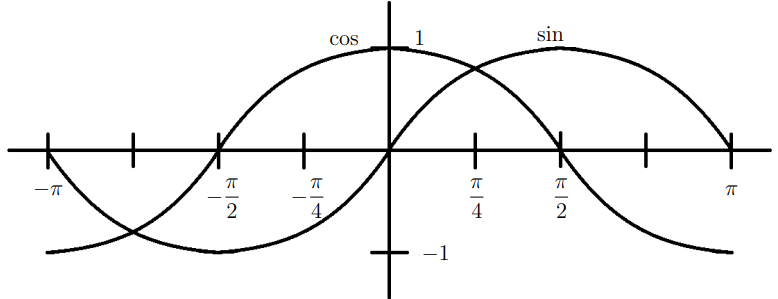
\includegraphics[width=\linewidth,keepaspectratio]{pictures/sinus_cosinus.png} 
\end{figure}

\begin{figure}[H]
 \centering
 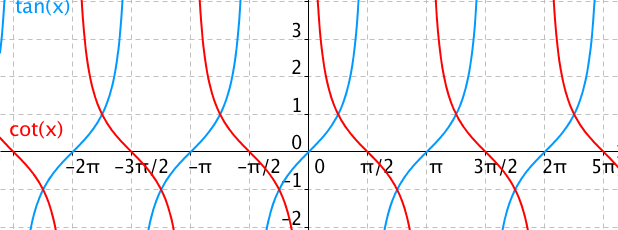
\includegraphics[width=\linewidth,keepaspectratio]{pictures/tan_cot.png} 
\end{figure}

\mysubsection{Hyperbel und Areafunktionen}
\DEF{Cosinus Hyperbolicus}{$cosh(x)=\frac{e^x+e^{-x}}{2}$.}

\DEF{Sinus Hyperbolicus}{$sinh(x)=\frac{e^x-e^{-x}}{2}$.}

\DEF{Tangens Hyperbolicus}{$tanh(x)=\frac{sinh(x)}{cosh(x)}=\frac{e^x-e^{-x}}{e^x+e^{-x}}$.}

\DEF{Arcosh}{$arcosh:[1,\infty)\rightarrow[0,\infty)$ bezeichnet die Umkehrfunktion von $cosh:[0,\infty)\rightarrow[1,\infty)$. Also $arcosh:=cosh^{-1}$.}

\DEF{Arsinh}{$arsinh:\mathbb{R}\rightarrow\mathbb{R}$ bezeichnet die Umkehrfunktion von $sinh:\mathbb{R}\rightarrow\mathbb{R}$. Also $arsinh:=sinh^{-1}$.}

\DEF{Artanh}{$artanh:(-1,1)\rightarrow\mathbb{R}$ bezeichnet die Umkehrfunktion von $tanh:\mathbb{R}\rightarrow(-1,1)$. Also $artanh:=tanh^{-1}$.}

\SA{}{
\begin{enumerate}
    \item $cosh^2(x)-sinh^2(x)=1\ \forall x\in\mathbb{R}$.
    \item $cosh(2x)=cosh^2(x)+sinh^2(x)$.
    \item $sinh(2x)=2sinh(x)cosh(x)$.
\end{enumerate}}

\begin{figure}[H]
 \centering
 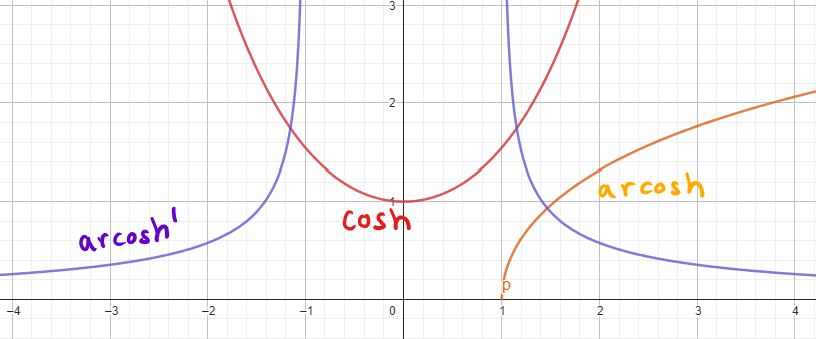
\includegraphics[width=\linewidth,keepaspectratio]{pictures/hyperbolic_cosinus.png} 
\end{figure}

\begin{figure}[H]
 \centering
 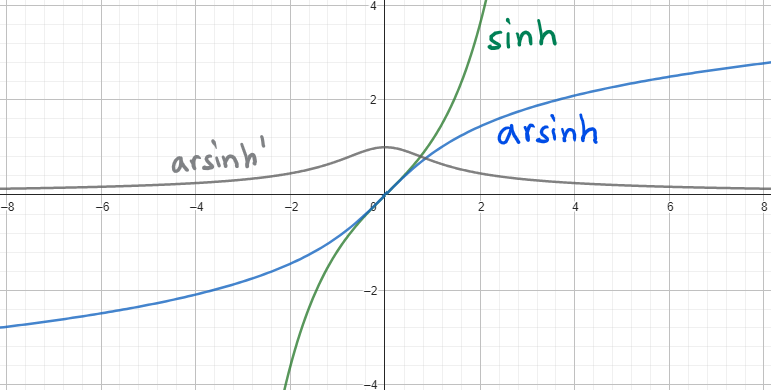
\includegraphics[width=\linewidth,keepaspectratio]{pictures/hyperbolic_sinus.png} 
\end{figure}

\mysubsection{Grenzwerte von Funktionen}
\DEF{Häufungspunkt}{Sei $D\subseteq\mathbb{R}$. Ein Häufungspunkt von $D$ ist eine Zahl $x_0\in\mathbb{R}$ oder $x_0=\infty$ oder $x_0=-\infty$ s.d. $\exists (a_n)_{n\geq 1}$ in $D\setminus \{x_0\}$ mit $lim_{n\rightarrow\infty}a_n=x_0$.

Umformulierungen:
\begin{itemize}
    \item Fall $x_0\in\mathbb{R}:$ $\forall\delta > 0:((x_0-\delta,x_0+\delta)\setminus \{x_0\})\cap D\not=\emptyset$.
    \item Fall $x_0=\infty:$ $\forall c>0: (c,\infty)\cap D\not=\emptyset$.
    \item Fall $x=-\infty:$ $\forall c>0: (-\infty,-c)\cap D\not = \emptyset$.
\end{itemize}}

\EXAMPLE{3.10.2}{Sei $D=\{0\}\cup(1,2)$. Dann ist $D'=[1,2]$ die Menge aller Häufungspunkte von $D$ und $0$ ist ein isolierter Punkt von $D$.}

\DEF{Existenz des Grenzwerts}{Sei $f:D\rightarrow\mathbb{R}$, $x_0$ ein Häufungspunkt von $D$, $A\in\mathbb{R}$ oder $A=\infty$ oder $A=-\infty$. Dann $lim_{x\rightarrow x_0}f(x)=A$ $\Leftrightarrow$ $\forall (a_n)_{n\geq 1}$ in $D\setminus\{x_0\}:$ $(lim_{n\rightarrow\infty}a_n=x_0 \Rightarrow lim_{n\rightarrow\infty}f(a_n)=A)$.

Falls kein solches $A$ existiert, sagen wir, der Grenzwert von $f$ für $x\rightarrow x_0$ existiert nicht.

Umformulierungen:
\begin{enumerate}
    \item Fall $x\in\mathbb{R}$ und $A\in\mathbb{R}$\\
            $lim_{x\rightarrow x_0}f(x)=A$ $\Leftrightarrow$ $\forall\varepsilon >0\ \exists\delta >0:\forall x\in ((x_0-\delta,x_0+\delta)\setminus \{x_0\})\cap D: |f(x)-A| < \varepsilon$.
    \item Fall $x\in\mathbb{R}$ und $A=-\infty$
            $lim_{x\rightarrow x_0}f(x)=A$ $\Leftrightarrow$ $\forall c >0\ \exists\delta >0:\forall x\in ((x_0-\delta,x_0+\delta)\setminus \{x_0\})\cap D: f(x) < -c$.
    \item Fall $x=-\infty$ und $A\in\mathbb{R}$
            $lim_{x\rightarrow x_0}f(x)=A$ $\Leftrightarrow$ $\forall\varepsilon >0\ \exists N >0:\forall x < -N, x\in D: |f(x)-A| < \varepsilon$.
    \item[...] Es gibt noch $6$ weitere Umformulierungen nach dem selben Schema.
\end{enumerate}}

\NOTE{3.10.4.2}{Sei $x_0\in D$. Dann $f$ stetig in $x_0$ $\Leftrightarrow lim_{x\rightarrow x_0}f(x)=f(x_0)$.}

\EXAMPLE{}{Sei $f:[0,2]\rightarrow\mathbb{R}$, $f(x)=\begin{cases}
    0 & x\in[0,1)\cup (1,2],\\
    1 & x=1.
\end{cases}$ Dann ist $lim_{x\rightarrow 1}f(x)=0\not = f(1)=1$ und $f$ ist nicht stetig in $x_0$. Merke: Wenn $x_0\not\in D$, dann kann $f:D\rightarrow\mathbb{R}$ in diesem Punkt nicht stetig sein.}

\DEF{Stetige Fortsetzung einer Funktion}{Wenn $x_0\not\in D$ und $lim_{x\rightarrow x_0}f(X)$ in $\mathbb{R}$ existiert, dann ist $f^{\sim}=\begin{cases}
    f(x) & x\in D,\\
    lim_{x\rightarrow x_0}f(x) & x=x_0
\end{cases}$ die stetige Fortsetzung von $f$, welche stetig in $x_0$ ist.}

\NOTE{3.10.4.3-5}{
\begin{enumerate}
    \item Sei $f,g:D\rightarrow\mathbb{R}$ und $lim_{x\rightarrow x_0}f(x),lim_{x\rightarrow x_0}g(x)$ existieren. Dann \begin{itemize}
    \item $lim_{x\rightarrow x_0}(f+g)(x)=lim_{x\rightarrow x_0}f(x)+lim_{x\rightarrow x_0}g(x)$.
    \item $lim_{x\rightarrow x_0}(f\cdot g)(x)=lim_{x\rightarrow x_0}f(x) \cdot lim_{x\rightarrow x_0}g(x)$.
    \end{itemize}
    \item Sei $f,g:D\rightarrow\mathbb{R}$, $f\leq g$, und beide Grenzwerte existieren. Dann $lim_{x\rightarrow x_0}f(x)\leq lim_{x\rightarrow x_0}g(x)$.
    \item Falls $g_1\leq f \leq g_2$ und $lim_{x\rightarrow x_0}g_1(x)=lim_{x\rightarrow x_0}g_2(x)$. Dann $\exists lim_{x\rightarrow x_0}f(x)$ und $lim_{x\rightarrow x_0}f(x)=lim_{x\rightarrow x_0}g_1(x)$.
\end{enumerate}}

\SA{3.10.6}{Seien $D,E\subseteq\mathbb{R}$, $x_0$ Häufungspunkt von $D$, $f:D\rightarrow E$. Angenommen $y_0:=lim_{x\rightarrow x_0}f(x)$ existiert und $y_0\in E$. $g:E\rightarrow\mathbb{R}$ stetig in $y_0$ $\Rightarrow lim_{x\rightarrow x_0}g(f(x))=g(y_0)$.}

\mysubsection{Links- und Rechtsseitige Grenzwerte}
\DEF{Rechtsseitiger Häufungspunkt und Grenzwert}{Sei $f:D\rightarrow\mathbb{R}$, $x_0\in\mathbb{R}$ ein Häufungspunkt von $D\cap(x_0,\infty)$. Dann ist $x_0$ ein rechtsseitiger Häufungspunkt.

Falls der Grenzwert von $f|_{D\cap[x_0,\infty)}$ für $x\rightarrow x_0$ existiert, wird er mit $lim_{x\rightarrow x_0^+}f(x)$ bezeichnet und nennt sich rechtsseitiger Grenzwert von $f$ bei $x_0$.

Falls $\forall\varepsilon > 0\ \exists\delta > 0: \forall x\in (x_0,x_0+\delta)\cap D: f(x) > \frac{1}{\varepsilon}$ $\Rightarrow lim_{x\rightarrow x_0^+}f(x)=\infty$.}


\DEF{Linksseitiger Häufungspunkt und Grenzwert}{Sei $f:D\rightarrow\mathbb{R}$, $x_0\in\mathbb{R}$ ein Häufungspunkt von $D\cap(-\infty, x_0)$. Dann ist $x_0$ ein linksseitiger Häufungspunkt.

Falls der Grenzwert von $f|_{D\cap(-\infty,x_0]}$ für $x\rightarrow x_0$ existiert, wird er mit $lim_{x\rightarrow x_0^-}f(x)$ bezeichnet und nennt sich linksseitiger Grenzwert von $f$ bei $x_0$.

Falls $\forall\varepsilon > 0\ \exists\delta > 0: \forall x\in (x_0,x_0+\delta)\cap D: f(x) < -\frac{1}{\varepsilon}$ $\Rightarrow lim_{x\rightarrow x_0^-}f(x)=\infty$.}

\SA{}{Sei $D\subseteq\mathbb{R},f:D\rightarrow\mathbb{R}$ und $x_0$ ein links- und rechtsseitiger Häufungspunkt von $D$. Dann $\exists\ lim_{x\rightarrow x_0}f(x)\Leftrightarrow(\exists\ lim_{x\rightarrow x_0^+}f(x) \land\exists\ lim_{x\rightarrow x_0^-}f(x)\land lim_{x\rightarrow x_0^+}f(x)=lim_{x\rightarrow x_0^-}f(x))$.}








\mysection[Dandelion]{\centering Differenzierbare Funktionen}
Sei $D\subseteq\mathbb{R},f:D\rightarrow\mathbb{R},x_0\in D$ Häufungspunkt von $D$.

\DEF{Differenzen-Quotient}{Der Differenzen-Quotient $\frac{\Delta f}{\Delta x}=\frac{f(x)-f(x_0)}{x-x_0}$ ist die Steigung der Geraden durch $(x_0,f(x_0)),(x,f(x))$.}

\begin{figure}[H]
 \centering
 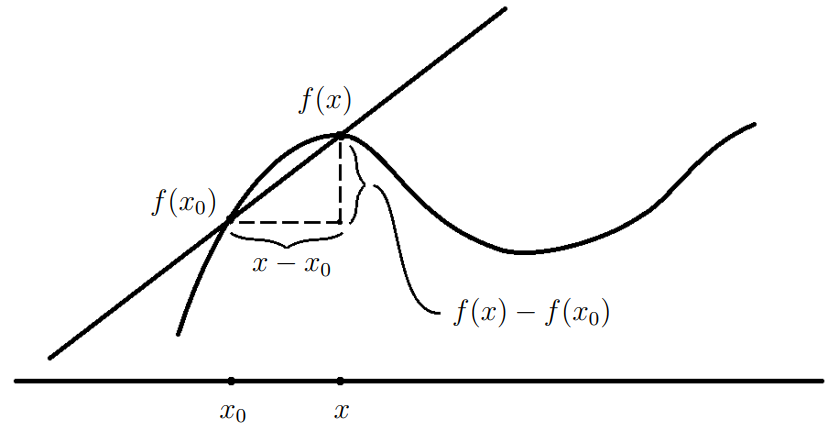
\includegraphics[width=\linewidth,keepaspectratio]{pictures/differenzen_quotient.png} 
\end{figure}

\DEF{Differenzierbar}{$f$ ist in $x_0$ differenzierbar, falls $\exists\ f'(x_0):=lim_{x\rightarrow x_0}\frac{f(x)-f(x_0)}{x-x_0}$.}

\NOTE{4.1.2}{Oftmals wird $f'(x_0)$ mit $x=x_0+h$ geschrieben: $f'(x_0)=lim_{h\rightarrow 0}\frac{f(x_0+h)-f(x_0)}{h}$.}

\SA{4.1.3}{Folgende Aussagen sind äquivalent:
\begin{enumerate}
    \item $f$ ist in $x_0$ differenzierbar.
    \item $\exists\ c\in\mathbb{R},\ r:D\rightarrow\mathbb{R}:$
    \begin{enumerate}
        \item[2.1] $f(x)=f(x_0)+c(x-x_0)+r(x)(x-x_0)$,
        \item[2.2] $r(x_0)=0 \land r$ stetig in $x_0$.
    \end{enumerate}
\end{enumerate}
Aus 2.1 folgt, dass $y=f(x_0)+f'(x_0)(x-x_0)$ die Gleichung der Tangente zum Graph von $f$ in $(x_0,f(x_0))$ ist. Wir können 2.1 noch Vereinfachen durch $\phi(x)=f'(x_0)+r(x)$.}

\SA{4.1.4}{$f$ in $x_0$ differenzierbar $\Leftrightarrow$ $\exists\ \phi:D\rightarrow\mathbb{R}$ die in $x_0$ stetig mit $f(x)=f(x_0)+\phi(x)(x-x_0)\ \forall x\in D$. Dann gilt $\phi(x_0)=f'(x_0)$.}

\COR{4.1.5}{$f$ in $x_0$ differenzierbar $\Rightarrow$ $f$ in $x_0$ stetig.}

\EXAMPLE{4.1.6}{
\begin{enumerate}
    \item $f=1:\mathbb{R}\rightarrow\mathbb{R},$ dann $f(x)-f(x_0)=1-1=0 \Rightarrow f'(x_0)=0\ \forall x_0\in\mathbb{R}$.
    \item $f:\mathbb{R}\rightarrow\mathbb{R},x\mapsto x,$ dann $f(x)-f(x_0)=x-x_0 \Rightarrow f'=1$.
    \item $f:\mathbb{R}\rightarrow\mathbb{R},x\mapsto x^2,$ dann $f(x)-f(x_0)=x^2-x_0^2=(x-x_0)(x+x_0)$. Somit für $x\not = x_0: \frac{f(x)-f(x_0)}{x-x_0}=x+x_0 \Rightarrow lim_{x\rightarrow x_0}\frac{f(x)-f(x_0)}{x-x_0}=lim_{x\rightarrow x_0}(x+x_0)=2x_0=f'(x_0)\ \forall x_0\in\mathbb{R}$.
    \item .
    \item .
\end{enumerate}}

\DEF{4.1.7}{$f:D\rightarrow\mathbb{R}$ ist in $D$ differenzierbar, falls $\forall$ Häufungspunkte $x_0\in D$, $f$ in $x_0$ differenzierbar.}

\EXAMPLE{4.1.8/10/13}{
\begin{enumerate}
    \item $(x^n)'=nx^{n-1}\ \forall n\geq 1,\ \forall x\in\mathbb{R}$.
    \item $exp'=exp$.
    \item $ln'(x)=\frac{1}{x}$.
    \item $sin'=cos$, $cos'=-sin$.
    \item $tan'(x)=\frac{1}{cos^2(x)}\ \forall x\not\in\frac{\pi}{2}+\pi\mathbb{Z}$.
    \item $cot'(x)=\frac{-1}{sin^2(x)}\ \forall x\not\in\pi\mathbb{Z}$.
    \item $arcsin'(x)=\frac{1}{\sqrt{1-x^2}}\ \forall x\in(-1,1)$.
    \item $arccos'(x)=\frac{-1}{\sqrt{1-x^2}}\ \forall x\in(-1,1)$.
    \item $arctan'(x)=\frac{1}{1+x^2}\ \forall x\in(-\infty,\infty)$.
    \item $arccot'(x)=\frac{-1}{1+x^2}\ \forall x\in(-\infty,\infty)$.
    \item $cosh'(x)=sinh(x)$, $sinh'(x)=cosh(x)$.
    \item $arcosh'(x)=\frac{1}{\sqrt{x^2-1}}\ \forall x\in(1,\infty)$.
    \item $arsinh'(x)=\frac{1}{\sqrt{x^2+1}}\ \forall x\in\mathbb{R}$.
    \item $artanh'(x)=\frac{1}{1-y^2}\ \forall y\in(-1,1).$
\end{enumerate}}

\SA{4.1.9}{Sei $D\subseteq\mathbb{R}, x_0\in D$ Häufungspunkt von $D$, $f,g:D\rightarrow\mathbb{R}$ in $x_0$ differenzierbar, $c\in\mathbb{R}$ konstant. Dann
\begin{enumerate}
    \item $c\cdot f,f+g$ in $x_0$ differenzierbar und 
    $(c\cdot f)'(x_0)=c\cdot f'(x_0)$, $(f+g)'(x_0)=f'(x_0)+g'(x_0)$.
    \item $f\cdot g$ in $x_0$ differenzierbar und $(f\cdot g)'(x_0)=f'(x_0)g(x_0)+f(x_0)g'(x_0)$.
    \item Falls $g(x_0)\not = 0$ ist $\frac{f}{g}$ in $x_0$ differenzierbar und $(\frac{f}{g})'(x_0)=\frac{f'(x_0)g(x_0)-f(x_0)g'(x_0)}{g(x_0)^2}$.
\end{enumerate}}


\SA{4.1.11 (Kettenregel)}{Seien $D,E\subseteq\mathbb{R}, x_0\in D$ ein Häufungspunkt. Sei $f:D\rightarrow E$ in $x_0$ differenzierbar s.d. $y_0:=f(x_0)$ ein Häufungspunkt von $E$. Sei $g:E\rightarrow\mathbb{R}$ eine in $y_0$ differenzierbare Funktion. Dann $g\circ f:D\rightarrow\mathbb{R}$ in $x_0$ differenzierbar und $(g\circ f)'(x_0)=g'(f(x_0))f'(x_0)$.}

\COR{4.1.12}{Sei $f:D\rightarrow E$ bijektiv, $x_0\in D$ Häufungspunkt. Angenommen $f$ in $x_0$ differenzierbar, $f'(x_0)\not = 0$, und $f^{-1}$ in $y_0=f(x_0)$ stetig. Dann $y_0$ Häufungspunkt von $E$, $f^{-1}$ in $y_0$ differenzierbar und $(f^{-1})'(y_0)=\frac{1}{f'(x_0)}$.}

\DEF{Lokale Maxima/Minima}{Sei $D\subseteq\mathbb{R},f:D\rightarrow\mathbb{R},x_0\in D$.
\begin{enumerate}
    \item $\exists\delta > 0: f(x)\leq f(x_0)\ \forall x\in (x-\delta,x+\delta)\cap D$ $\Rightarrow x_0$ ist lokales Maximum von $f$.
    \item $\exists\delta > 0: f(x)\geq f(x_0)\ \forall x\in (x-\delta,x+\delta)\cap D$ $\Rightarrow x_0$ ist lokales Minimum von $f$.
    \item $x_0$ lokales Maximum $\lor$ $x_0$ lokales Minumum $\Rightarrow x_0$ lokales Extremum.
\end{enumerate}}

\DEF{Example}{Sei $f:[a,b]\rightarrow\mathbb{R}$ wie im nachfolgenden Bild. Dann sind $a,x_1,x_3$ lokale Minima und $x_0,x_2,b$ lokale Maxima.}
\begin{figure}[H]
 \centering
 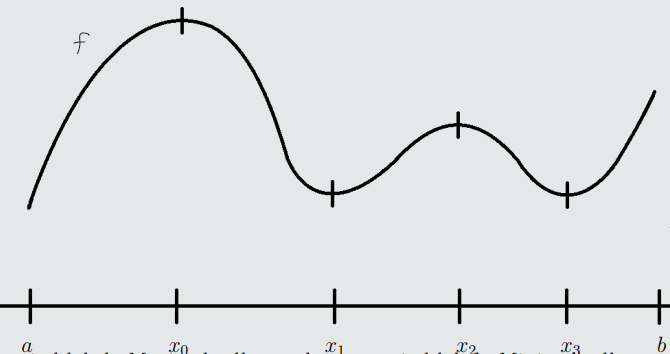
\includegraphics[width=\linewidth,keepaspectratio]{pictures/lokale_maxima_und_minima.png} 
\end{figure}

\DEF{Ableitungen von geraden und ungeraden Funktionen}{Sei $f:\mathbb{R}\rightarrow\mathbb{R}$. 

$f$ gerade $\Leftrightarrow f(-x)=f(x)\ \forall x\in\mathbb{R} \Rightarrow f'$ ungerade.

$f$ ungerade $\Leftrightarrow f(-x)=-f(x)\ \forall x\in\mathbb{R} \Rightarrow f'$ gerade.}


\SA{4.2.2}{Sei $D\subseteq\mathbb{R},x_0\in D$ Häufungspunkt von $D$, $f:D\rightarrow\mathbb{R}$ differenzierbar in $x_0$.
\begin{enumerate}
    \item $f'(x_0)>0\Rightarrow\ \exists\delta > 0:$\\
            $f(x)>f(x_0)\ \forall x\in (x_0,x_0+\delta)\cap D$,\\
            $f(x)<f(x_0)\ \forall x\in (x_0-\delta,x_0)\cap D$.
    \item $f'(x_0)<0\Rightarrow\ \exists\delta > 0:$\\
            $f(x)<f(x_0)\ \forall x\in (x_0,x_0+\delta)\cap D$,\\
            $f(x)>f(x_0)\ \forall x\in (x_0-\delta,x_0)\cap D$.
    \item $f$ besitzt lokales Extremum in $x_0$ $\land$ $x_0$ ist links- und rechtsseitiger Häufungspunkt von $D$ $\Rightarrow f'(x_0)=0$.
\end{enumerate}}

\SA{4.2.3 (Rolle 1690)}{Sei $a<b$, $f:[a,b]\rightarrow\mathbb{R}$ stetig und in $(a,b)$ differenzierbar. Wenn $f(a)=f(b) \Rightarrow\ \exists \xi\in(a,b)$ mit $f'(\xi)=0$.}

\SA{4.2.4 (Mittelwertsatz, Lagrange 1797)}{Sei $a<b$, $f:[a,b]\rightarrow\mathbb{R}$ stetig und in $(a,b)$ differenzierbar. Dann $\exists\ \xi\in(a,b)$ mit $f(b)-f(a)=f'(\xi)(b-a)\Leftrightarrow f'(\xi)=\frac{f(b)-f(a)}{b-a}$.}

\COR{4.2.5}{Sei $a<b,f,g:[a,b]\rightarrow\mathbb{R}$ stetig und in $(a,b)$ differenzierbar.
\begin{enumerate}
    \item $f'(\xi)=0\ \forall\xi\in(a,b) \Rightarrow f$ konstant.
    \item $f'(\xi)=g'(\xi)\ \forall\xi\in(a,b) \Rightarrow\exists c\in\mathbb{R}:f(x)=g(x)+c\ \forall x\in[a,b]$.
    \item $f'(\xi)\geq 0\ \forall\xi\in(a,b) \Rightarrow f$ auf $[a,b]$ monoton wachsend.
    \item $f'(\xi)>0\ \forall\xi\in(a,b) \Rightarrow f$ auf $[a,b]$ streng monoton wachsend.
    \item $f'(\xi)< 0\ \forall\xi\in(a,b) \Rightarrow f$ auf $[a,b]$ monoton fallend.
    \item $f'(\xi)\leq0\ \forall\xi\in(a,b) \Rightarrow f$ auf $[a,b]$ streng monoton fallend.
    \item $\exists M\geq 0:|f'(\xi)|\leq M\ \forall\xi\in(a,b) \Rightarrow \forall x_1,x_2\in[a,b]:|f(x_1)-f(x_2)|\leq M|x_1-x_2|$.
\end{enumerate}}

\SA{4.2.9 (Cauchy)}{Seien $a<b,f,g:[a,b]\rightarrow\mathbb{R}$ stetig und in $(a,b)$ differenzierbar. Dann $\exists \xi\in(a,b):g'(\xi)(f(b)-f(a))=f'(\xi)(g(b)-g(a))$. Falls $g'(x)\not = 0\ \forall x\in(a,b)$ $\Rightarrow g(a)\not = g(b) \land \frac{f(b)-f(a)}{g(b)-g(a)}=\frac{f'(\xi)}{g'(\xi)}$.}

\SA{4.2.10 (l'Hospital)}{Seien $a<b,f,g:(a,b)\rightarrow\mathbb{R}$ differenzierbar mit $g'(x)\not = 0\ \forall x\in(a,b)$. Falls $(lim_{x\rightarrow b^-}f(x)=lim_{x\rightarrow b^-}g(x)=0$ $\lor$ $(lim_{x\rightarrow b^-}f(x)= \pm\infty \land lim_{x\rightarrow b^-}g(x)=\pm\infty))$ $\land$ $\exists lim_{x\rightarrow b^-}\frac{f'(x)}{g'(x)}=:\lambda$ $\Rightarrow lim_{x\rightarrow b^-}\frac{f(x)}{g(x)}=lim_{x\rightarrow b^-}\frac{f'(x)}{g'(x)}$.

Der Satz gilt auch falls \begin{itemize}
    \item $b=\infty$,
    \item $a=-\infty$,
    \item $\lambda = \pm\infty$,
    \item $x\rightarrow a^+$.
\end{itemize}}

\DEF{Konvex}{Sei $I\subseteq\mathbb{R}$ ein Intervall mit mehr als einem Punkt und $f:I\rightarrow\mathbb{R}$.
\begin{enumerate}
    \item $x,y \in I, \forall x\leq y, \lambda\in[0,1]:f(\lambda x+(1-\lambda)y)\leq\lambda f(x)+(1-\lambda)f(y)$ $\Rightarrow f$ konvex auf $I$.
    \item $x,y \in I, \forall x<y, \lambda\in[0,1]:f(\lambda x+(1-\lambda)y)<\lambda f(x)+(1-\lambda)f(y)$ $\Rightarrow f$ streng konvex auf $I$.
\end{enumerate}}

\begin{figure}[H]
 \centering
 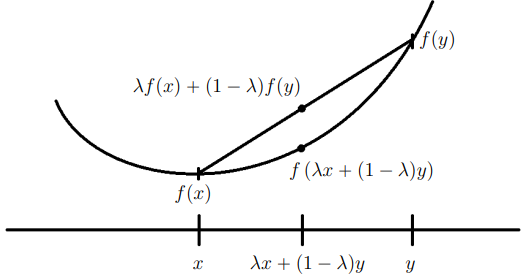
\includegraphics[width=\linewidth,keepaspectratio]{pictures/konvex.png} 
\end{figure}

\DEF{Konkav}{Sei $I\subseteq\mathbb{R}$ ein Intervall mit mehr als einem Punkt und $f:I\rightarrow\mathbb{R}$.

$-f$ (streng) konvex $\Rightarrow$ $f$ (streng) konkav.}

\NOTE{4.2.14}{Sei $f:I\rightarrow\mathbb{R}$ konvex. $\forall n\geq 1, \{x_1,...,x_n\}\subseteq I, \lambda_1,...,\lambda_n\in[0,1]$ mit $\sum_{i=1}^n\lambda_i=1$ gilt $f(\sum_{i=1}^n\lambda_ix_i)\leq\sum_{i=1}^n\lambda_if(x_i)$.}

\LEM{4.2.15}{Sei $f:I\rightarrow\mathbb{R}$ beliebig. Dann 
\begin{enumerate}
    \item $f$ konvex $\Leftrightarrow$ $\forall x_0<x<x_1\in I:$ $\frac{f(x)-f(x_0)}{x-x_0}\leq\frac{f(x_1)-f(x)}{x_1-x}$,
    \item $f$ streng konvex $\Leftrightarrow$ $\forall x_0<x<x_1\in I:$ $\frac{f(x)-f(x_0)}{x-x_0}<\frac{f(x_1)-f(x)}{x_1-x}$,
    \item $f$ konkav $\Leftrightarrow$ $\forall x_0<x<x_1\in I:$ $\frac{f(x)-f(x_0)}{x-x_0}\geq\frac{f(x_1)-f(x)}{x_1-x}$,
    \item $f$ streng konkav $\Leftrightarrow$ $\forall x_0<x<x_1\in I:$ $\frac{f(x)-f(x_0)}{x-x_0}>\frac{f(x_1)-f(x)}{x_1-x}$.
\end{enumerate}}

\LEM{}{Sei $f:I\rightarrow\mathbb{R}$ und $x_0<x<x_1\in I$. Dann folgt aus L4.2.15: 
\begin{enumerate}
    \item $f$ konvex $\Rightarrow$ $\frac{f(x)-f(x_0)}{x-x_0}\leq\frac{f(x_1)-f(x_0)}{x_1-x_0}\leq\frac{f(x_1)-f(x)}{x_1-x}$. 
    \item $f$ konkav $\Rightarrow$ $\frac{f(x)-f(x_0)}{x-x_0}\geq\frac{f(x_1)-f(x_0)}{x_1-x_0}\geq\frac{f(x_1)-f(x)}{x_1-x}$. 
\end{enumerate}
Strenge Konvexität (Konkavität) impliziert $<$ ($>$) statt $\leq$ ($\geq$) in obigen Ungleichungen.}

\SA{4.2.16}{Seien $a<b$. Sei $f:(a,b)\rightarrow\mathbb{R}$ in $(a,b)$ differenzierbar. Dann
\begin{enumerate}
    \item $f$ (streng) konvex $\Leftrightarrow$ $f'$ (streng) monoton steigend, 
    \item $f$ (streng) konkav $\Leftrightarrow$ $f'$ (streng) monoton fallend.
\end{enumerate}
Gilt auch für geschlossene Intervalle.}

\COR{4.2.17}{Seien $a<b$. Sei $f:(a,b)\rightarrow\mathbb{R}$ in $(a,b)$ zweimal differenzierbar. Dann
\begin{enumerate}
    \item $f''\geq 0$ (bzw. $f''>0$) auf $(a,b)$ $\Rightarrow$ $f$ (streng) konvex,
    \item $f''\leq 0$ (bzw. $f''<0$) auf $(a,b)$ $\Rightarrow$ $f$ (streng) konkav.
\end{enumerate}}


\mysubsection{Höhere Ableitungen}
Sei $D\subseteq\mathbb{R}$ s.d jedes $x_0\in D$ Häufungspunkt von $D$ ist. Sei $f:D\rightarrow\mathbb{R}$ differenzierbar in $D$ und $f^{(1)}=f'$ ihre Ableitung.

\DEF{Höhere Ableitungen}{
\begin{enumerate}
    \item Für $n\geq 2$ ist $f$ n-mal differenzierbar in $D$ falls $f^{(n-1)}$ in $D$ differenzierbar. Dann ist $f^{(n)}:=(f^{(n-1)})'$ die $n$-te Ableitung von $f$.
    \item $f$ $n$-mal differenzierbar $\land\ f^{(n)}$ in $D$ stetig $\Rightarrow f$ $n$-mal stetig differenzierbar in $D$.
    \item $f\ \forall n\geq 1$ $n$-mal differenzierbar $\Rightarrow$ $f$ ist in $D$ glatt (smooth).
\end{enumerate}}

\NOTE{4.3.2}{Für $n\geq 1:$ $f$ $n$-mal differenzierbar $\Rightarrow$ $f\ (n-1)$-mal stetig differenzierbar. Somit sind glatte Funktionen $n$-mal stetig differenzierbar $\forall n\geq 1$.}

\EXAMPLE{4.3.4/7}{
\begin{enumerate}
    \item $exp,sin,cos,sinh,cosh,tanh$ sind glatt auf ganz $\mathbb{R}$.
    \item $tan$ ist auf $\mathbb{R}\setminus\{\frac{\pi}{2}+k\pi:k\in\mathbb{Z}\}$ glatt.
    \item $cot$ ist auf $\mathbb{R}\setminus\{k\pi:k\in\mathbb{Z}\}$ glatt.
    \item $arcsin, arccos, arctan, arccot$ sind glatt.
    \item Polynome sind auf ganz $\mathbb{R}$ glatt.
    \item $ln:(0,\infty)\rightarrow\mathbb{R}$ ist glatt. Es gilt $ln^{(n)}(x)=(-1)^{n-1}(n-1)!x^{-n}\ \forall n\geq 1$.
    \item $sqrt:[0,\infty)\rightarrow[0,\infty)$ ist glatt auf $(0,\infty)$.
\end{enumerate}}

\SA{4.3.3}{Sei $n\geq 1$. Sei $f,g:D\rightarrow\mathbb{R}$ $n$-mal differenzierbar in $D$. Dann
\begin{enumerate}
    \item $f+g$ ist $n$-mal differenzierbar und $(f+g)^{(n)}=f^{(n)}+g^{(n)}$.
    \item $f\cdot g$ ist $n$-mal differenzierbar und $(f\cdot g)^{(n)}=\sum_{k=0}^n{n\choose k}f^{(k)}g^{(n-k)}$.
\end{enumerate}}

\SA{4.3.5}{Sei $n\geq 1$. Sei $f,g:D\rightarrow\mathbb{R}$ $n$-mal differenzierbar in $D$. Sei $g(x)\not = 0$ $\forall x\in D$. Dann $\frac{f}{g}$ $n$-mal differenzierbar in $D$.}

\SA{4.3.6}{Seien $E,D\subseteq\mathbb{R}$ Teilmengen für die jeder Punkt Häufungspunkt ist. Seien $f:D\rightarrow\mathbb{E}$ und $g:E\rightarrow\mathbb{R}$ $n$-mal differenzierbar. Dann ist $g\circ f$ $n$-mal differenzierbar, und $(g\circ f)^{(n)}(x)=\sum_{k=1}^nA_{n,k}(x)(g^{(k)}\circ f)(x)$ wobei $A_{n,k}$ ein Polynom in den Funktionen $f',f^{(2)},...,f^{(n+1-k)}$ ist. Beispiele:

\begin{itemize}
    \item $(g\circ f)'=(g'\circ f)f'$.
    \item $(g\circ f)^{(2)}=(g^{(2)}\circ f)(f')^2+(g'\circ f)f^{(2)}$.
    \item $(g\circ f)^{(3)}=(g^{(3)}\circ f)(f')^3+3(g^{(2)}\circ f)f'f^{(2)}+(g'\circ f)f^{(3)}$.
\end{itemize}}

\mysubsection{Potenzreihen, Taylor Approximation}
\SA{4.4.1}{Sei $I\subseteq\mathbb{R}$. Seien $f_n:I\rightarrow\mathbb{R}$, $n\in\mathbb{N}^*$, stetig differenzierbar. Angenommen
\begin{enumerate}
    \item $(f_n)_{n\geq 1}$ konvergiert gleichmässig in $I$ gegen $lim_{n\rightarrow\infty}f_n=:f$,
    \item $(f'_n)_{n\geq 1}$ konvergiert gleichmässig in $I$ gegen $lim_{n\rightarrow\infty}f'_n=:p$.
\end{enumerate}
Dann $f$ stetig differenzierbar und $f'=p$.}

\SA{4.4.2}{Sei $\sum_{k=0}^{\infty}c_kx^k$ eine Potenzreihe mit $\rho > 0$. Dann ist $f(x)=\sum_{k=0}^{\infty}c_k(x-x_0)^k$ auf $(x_0-\rho,x_0+\rho)$ differenzierbar und $f'(x)=\sum_{k=1}^{\infty}kc_k(x-x_0)^{k-1}\ \forall x\in(x_0-\rho,x_0+\rho)$.}

\COR{4.4.3}{Unter der Voraussetzung von Satz 4.4.1 ist $f$ auf $(x_0-\rho,x_0+\rho)$ glatt und $f^{(j)}(x)=\sum_{k=j}^{\infty}c_k\frac{k!}{(k-j)!}(x-x_0)^{k-j}$. Insbesondere ist $c_j=\frac{f^{(j)}(x_0)}{j!}$.}

\EXAMPLE{4.4.4}{Nicht jede glatte Funktion ist Summe einer Potenzreihe.}

\DEF{Taylorpolynom}{Sei $I\in\mathbb{R}$ ein Intervall mit mehr als einem Punkt. Sei $n\in\mathbb{N},f:I\rightarrow\mathbb{R}$ $n$-mal differenzierbar. Sei $x_0\in I$. Dann ist das Tylorpolynom der Ordnung $n$ von $f$ in $x_0:$ $T_nf(x;x_0):=\sum_{k=0}^n\frac{f^{(k)}(x_0)}{k!}(x-x_0)^k$. $p:=T_nf(x;x_0)$ ist eindeutig mit
\begin{enumerate}
    \item $Grad(p)\leq n$.
    \item $f(x_0)=p(x_0),\ f'(x_0)=p'(x_0),\ ...,\ f^{(n)}(x_0)=p^{(n)}(x_0)$.
\end{enumerate}}

\SA{4.4.5 (Approximation glatter Funktionen)}{Sei $f:[a,b]\rightarrow\mathbb{R}$ stetig und in $(a,b)$ $(n+1)$-mal differenzierbar. Sei $x_0\in[a,b]$. Dann $\forall x\in[a,b],x\not=x_0\ \exists\xi$ zwischen $x_0$ und $x$ mit $f(x)=T_nf(x;x_0)+\frac{f^{(n+1)}(\xi)}{(n+1)!}(x-x_0)^{n+1}$.}

\COR{4.4.6 (Taylor Approximation)}{Sei $f:[a,b]\rightarrow\mathbb{R}$ $n$-mal stetig differenzierbar und in $(a,b)$ $(n+1)$-mal differenzierbar. Sei $x_0\in[a,b]$. Dann $\forall x\in[a,b],x\not=x_0\ \exists\xi$ zwischen $x_0$ und $x$ s.d. $f(x)=T_nf(x;x_0)+\frac{f^{(n+1)}(\xi)}{(n+1)!}(x-x_0)^{n+1}$.}

\DEF{Restglied der Taylor Approximation}{$f(x)-T_nf(x;x_0)$ wird als Restglied bezeichnet. Die Formel $\frac{f^{(n+1)}(\xi)}{(n+1)!}(x-x_0)^{n+1}$ ist die Restglieddarstellung von Lagrange.}

\COR{4.4.7}{Sei $n\geq 0, a<x_0<b$ und $f:[a,b]\rightarrow\mathbb{R}$ in $(a,b)$ $(n+1)$-mal stetig differenzierbar. Angenommen $f'(x_0)=f^{(2)}(x_0)=...=f^{(n)}(x_0)=0$.
\begin{enumerate}
    \item $n$ gerade $\land$ $x_0$ lokales Extremum $\Rightarrow$ $f^{(n+1)}(x_0)=0$,
    \item $n$ ungerade $\land$ $f^{(n+1)}(x_0)>0$ $\Rightarrow$ $x_0$ strikte lokale Minimalstelle,
    \item $n$ ungerade $\land$ $f^{(n+1)}(x_0)<0$ $\Rightarrow$ $x_0$ strikte lokale Maximastelle.
\end{enumerate}}

\COR{4.4.8}{Sei $f:[a,b]\rightarrow\mathbb{R}$ stetig und in $(a,b)$ zweimal stetig differenzierbar. Sei $a<x_0<b$. Angenommen $f'(x_0)=0$.
\begin{enumerate}
    \item $f''(x_0)>0$ $\Rightarrow$ $x_0$ striktes lokales Minima,
    \item $f''(x_0)<0$ $\Rightarrow$ $x_0$ striktes lokales Maxima.
\end{enumerate}}

\mysection[JungleGreen]{\centering Riemann Integral}
\mysection[Aquamarine]{\centering Weiteres}
\mysubsection{Rechenregeln für Summen}
\begin{enumerate}
    \item $\sum_{i=L}^Ux_i=\sum_{i=L}^{I-1}x_i+\sum_{i=I}^Ux_i$
    \item $\sum_{i=L}^Ucx_i=c\sum_{i=L}^Ux_i$
    \item $\sum_{i=L}^Ux_i\pm\sum_{i=L}^Uy_i=\sum_{i=L}^U(x_i\pm y_i)$
    \item $\sum_{i=L_1}^{U_1}x_{i_1}\cdot ... \cdot \sum_{i=L_n}^{U_n}x_{i_n}=\sum_{i=L_1}^{U_1}\cdot ... \cdot \sum_{i=L_n}^{U_n}(x_{i_1}\cdot ...\cdot x_{i_n})$
    \item $\sum_{i=L_1}^{U_1}\sum_{j=L_2}^{U_2}x_{i,j}=\sum_{j=L_2}^{U_2}\sum_{i=L_1}^{U_1}x_{i,j}$
\end{enumerate}

\mysubsection{Summenformeln}
\begin{enumerate}
    \item $\sum_{i=1}^{n} i = 1 + 2 + 3 + ... + n = \frac{n(n+1)}{2} = \frac{1}{2}n^2 + \frac{1}{2}n$
    \item $\sum_{i=1}^{n} i^2 = 1^2 + 2^2 + 3^2 + ... + n^2 = \frac{n(n+1)(2n + 1)}{6} = \frac{1}{3}n^3 + \frac{1}{2}n^2 + \frac{1}{6}n$
    \item $\sum_{i=1}^{n} i^3 = 1^3 + 2^3 + 3^3 + ... + n^3 = \frac{n^2(n+1)^2}{4} = \frac{1}{4}n^4 + \frac{1}{2}n^3 + \frac{1}{4}n^2$
    \item $\sum_{k=0}^{n} aq^k = aq^0 + aq^1 + aq^2 + ... + aq^n = \frac{a(q^{n+1}-1)}{q-1}=\frac{a(1-q^{n+1})}{1-q}$
    \item $(j+1)^2 - j^2 = 2j + 1$
    \item $C_1 \cdot n^{k+1} \leq \sum_{i=1}^{n} i^k \leq C_2 \cdot n^{k+1}$ where $C_1 = \frac{1}{2^{k+1}}$ and $C_2 = 1$ are two constants independent of $n$. Hence, when n is large, $\sum_{i=1}^n i^k$ behaves "almost like $n^{k+1}$" up to a constant factor. In other words $\sum_{i=1}^n i^k = \theta (n^{k+1})$.
\end{enumerate}


\mysubsection{Grenzwerte}
\DEF{Asymptotisches Wachstumsverhalten}{$lim_{n\rightarrow\infty}:1<\log(\log(n))<\log(n)<\sqrt{n}<n<n\log(n)<n^2<2^n<n!<n^n$.}

\DEF{Wichtige Grenzwerte}{\begin{enumerate}
    \item $lim_{n\rightarrow\infty}(1 + \frac{1}{n})=1$.
    \item $lim_{n\rightarrow\infty}(1 + \frac{1}{n})^b=1^b=1$\hspace*{\fill}$ \forall b\in\mathbb{Z}$.
    \item $lim_{n\rightarrow\infty}n^aq^n=0$\hspace*{\fill}$ \forall a\in\mathbb{Z},0\leq q < 1$.
    \item $lim_{n\rightarrow\infty}(\frac{1}{1+\varepsilon})^n=0$\hspace*{\fill}$ \forall \varepsilon>0$.
    \item $lim_{n\rightarrow\infty}\sqrt[n]{a}=1$\hspace*{\fill}$ \forall a\in\mathbb{R},a>0$.
    \item $lim_{n\rightarrow\infty}(1+\frac{z}{n})^n=exp(z)$.
    \item $lim_{x\rightarrow 0^+}ln(x)=-\infty$.
    \item $lim_{x\rightarrow 0^+}x^a=0$\hspace*{\fill}$a>0$.
    \item $lim_{x\rightarrow 0}\frac{sin(x)}{x}=1$\hspace*{\fill}$ x\in D=\mathbb{R}\setminus\{0\}$.
    \item $lim_{x\rightarrow 0}\frac{cos(x)-1}{x}=0$.
\end{enumerate}}


\mysubsection{Reihen}
\DEF{Definitionen per Potenzreihe}{
\begin{enumerate}
    \item $exp(x)=\sum_{n=0}^{\infty}\frac{x^n}{n!}$\hspace*{\fill} $\rho=\infty$.
    \item $sin(x)=\sum_{n=0}^{\infty}(-1)^n\frac{x^{2n+1}}{(2n+1)!}$\hspace*{\fill} $\rho=\infty$.
    \item $cos(x)=\sum_{n=0}^{\infty}(-1)^{n}\frac{x^{2n}}{(2n)!}$\hspace*{\fill} $\rho=\infty$.
    \item $ln(x+1)=\sum_{n=0}^{\infty}(-1)^{n+1}\frac{x^n}{n}$\hspace*{\fill} $\rho=1$.
\end{enumerate}}

\DEF{Wichtige Reihen}{\begin{enumerate}
    \item $\sum_{n=0}^{\infty}\frac{1}{n}$ divergiert.
    \item $\sum_{n=0}^{\infty}\frac{1}{n^p}$ konvergiert $\forall p>1$.
    \item $\sum_{n=0}^{\infty}\frac{(-1)^n}{n}$ konvergiert, aber nicht absolut.
    \item $\sum_{n=0}^{\infty}\frac{1}{n^2}=\frac{\pi^2}{6}$.
    \item $\sum_{n=0}^{\infty}\frac{1}{n(n+1)}=1$.
    \item $\sum_{n=0}^{\infty}aq^n=\frac{a}{1-q}$\hspace*{\fill}$q\in\mathbb{C},|q|<0,a\in\mathbb{R}$.
\end{enumerate}}



\mysubsection{Uneigentliche Integrale}
\begin{enumerate}
    \item $\int_0^{\infty}e^{-x}dx=1$
    \item $\int_1^{\infty}\frac{1}{x^a}dx=\begin{cases}
    divergiert & \alpha\leq 1,\\
    \frac{1}{\alpha-1} & \alpha > 1.
    \end{cases}$
    \item $\int_0^1\frac{1}{x^a}dx=\begin{cases}
    divergiert & \alpha \geq 1,\\
    \frac{1}{1-\alpha} & \alpha < 1.
    \end{cases}$
\end{enumerate}


\mysubsection{Ableitungen}
\begin{center}
  % the c>{\centering\arraybackslash}X is a workaround to have a column fill up all space and still be centered
  \begin{tabularx}{\linewidth}{c>{\centering\arraybackslash}Xc}
  \toprule
  $\mathbf{F(x)}$ & $\mathbf{f(x)}$ & $\mathbf{f'(x)}$ \\
  \midrule
  $x$ & $c$ & $0$ \\[3px]
  $\frac{x^{c+1}}{c+1}$ & $x^c$ & $c \cdot x^{c-1}$ \\[3px]
  $\ln |x|$ & $\frac{1}{x}$ & $-\frac{1}{x^2}$ \\[3px]
  $\frac{x^{-c+1}}{-c+1}$ & $\frac{1}{x^c}$ & $\frac{-c}{x^{c+1}}$ \\[3px]
  $\frac{2}{3}x^{3/2}$ & $\sqrt{x}$ & $\frac{1}{2\sqrt{x}}$\\[3px]
  $\frac{1}{c \ln(a)}a^{cx}$ & $a^{cx}$ & $ca^{cx} \ln(a)$ \\[3px]
  $-\cos(x)$ & $\sin(x)$ & $\cos(x)$ \\[3px]
  $\sin(x)$ & $\cos(x)$ & $-\sin(x)$ \\[3px]
  $\frac{1}{2}(x-\frac{1}{2}\sin(2x))$ & $\sin^2(x)$ & $2 \sin(x)\cos(x)$ \\[3px]
  $\frac{1}{2}(x + \frac{1}{2}\sin(2x))$ & $\cos^2(x)$ & $-2\sin(x)\cos(x)$ \\[3px]
  $-\ln|\cos(x)|$ & $\tan{x}$ & $1+\tan^2(x)=\frac{1}{cos^2(x)}$\\[3px]
  $\ln | \sin(x)|$ & $\cot(x)$ & $\frac{-1}{\sin^2(x)}$ \\[3px]
  $\cosh(x)$ & $\sinh(x)$ & $\cosh(x)$ \\[3px]
  $\ln|\cosh(x)|$ & $\tanh(x)$ & $\frac{1}{\cosh^2(x)}$ \\[3px]
  $\frac{1}{c} \cdot e^{cx}$ & $e^{cx}$ & $c \cdot e^{cx}$ \\[3px]
  $x(\ln |x| - 1)$ & $\ln |x|$ & $\frac{1}{x}$ \\[3px]
  $\frac{1}{2}(\ln(x))^2$ & $\frac{\ln(x)}{x}$ & $\frac{1 - \ln(x)}{x^2}$ \\[3px]
  $\frac{x}{\ln(a)} (\ln|x| -1)$ & $\log_a |x|$ & $\frac{1}{\ln(a)x}$ \\[3px]
  $ $ & $\arcsin(x)$ & $\frac{1}{\sqrt{1-x^2}}$ \\[3px]
  $ $ & $\arccos(x)$ & $\frac{-1}{\sqrt{1-x^2}}$ \\[3px]
  $ $ & $\arctan(x)$ & $\frac{1}{1+x^2}$ \\[3px]
  $ $ & $\text{arccot}(x)$ & $\frac{-1}{1+x^2}$ \\[3px]
  $ $ & $\text{arsinh}(x)$ & $\frac{1}{\sqrt{x^2+1}}$ \\[3px]
  $ $ & $\text{arcosh}(x)$ & $\frac{-1}{\sqrt{x^2-1}}$ \\[3px]
  $ $ & $\text{artanh}(x)$ & $\frac{1}{1-x^2}$ \\[3px]
  \bottomrule
  \end{tabularx}
\end{center}


\mysubsection{Algebraische Gesetze}
\DEF{Quadratische Gleichungen Lösen}{$f(x)=ax^2+bx+c=0 \Rightarrow x=\frac{-b\pm\sqrt{D}}{2a}=\frac{-b\pm\sqrt{b^2-4ac}}{2a}$. \begin{itemize}
    \item $D=0\Rightarrow f$ hat eine Nullstelle
    \item $D>0\Rightarrow f$ hat zwei Nullstellen
    \item $D<0\Rightarrow f$ hat keine Nullstellen.
\end{itemize}}

\DEF{Faktorisierung spezieller Polynome}{
\begin{enumerate}
    \item $x^2-y^2=(x+y)(x-y)$
    \item $x^3+y^3=(x+y)(x^2-xy+y^2)$
    \item $x^3-y^3=(x-y)(x^2+xy+y^2)$
\end{enumerate}}

\DEF{Binomische Formel}{Für $n\in\mathbb{N}: (x+y)^n=\sum_{k=0}^n{n\choose k}x^{n-k}y^k$ wobei ${n\choose k}$ der Binomialkoeffizient "n tief k" ist: ${n\choose k}=\frac{n!}{k!(n-k)!}=\frac{n\cdot (n-1) \cdot (n-2) \cdot ... \cdot (n-k+1)}{k\cdot (k-1) \cdot ... \cdot 3 \cdot 2 \cdot 1}={n\choose n-k}$.

\begin{tabular}{>{$n=$}l<{\hspace{25pt}}*{13}{c@{\hspace{2pt}}}}
0 &&&&&&&1&&&&&&\\
1 &&&&&&1&&1&&&&&\\
2 &&&&&1&&2&&1&&&&\\
3 &&&&1&&3&&3&&1&&&\\
4 &&&1&&4&&6&&4&&1&&\\
5 &&1&&5&&10&&10&&5&&1&\\
6 &1&&6&&15&&20&&15&&6&&1
\end{tabular}}


\DEF{Potenzieren}{\begin{enumerate}
    \item $a^m\cdot a^n=a^{m+n}$
    \item $\frac{a^m}{a^n}=a^{m-n}=\frac{1}{a^{n-m}}$
    \item $(a^m)^n=a^{mn}=(a^n)^m$
    \item $a^n\cdot b^n=(ab)^n$
    \item $\frac{a^n}{b^n}=(\frac{a}{b})^n, b\not =0$
    \item $a^{-n}=\frac{1}{a^n} \Leftrightarrow a^{n}=\frac{1}{a^{-n}}$
\end{enumerate}}

\DEF{Radizieren}{
\begin{enumerate}
    \item $\sqrt[n]{a}\cdot\sqrt[n]{b}=\sqrt[n]{ab}$
    \item $\frac{\sqrt[n]{a}}{\sqrt[n]{b}}=\sqrt[n]{\frac{a}{b}},b\not=0$
    \item $\sqrt[n]{\sqrt[m]{a}}=\sqrt[n\cdot m]{a}$
    \item $a^{\frac{n}{m}}=\sqrt[m]{a^n}=\frac{1}{a^{-\frac{n}{m}}}$
\end{enumerate}}

\DEF{Logarithmieren}{
\begin{enumerate}
    \item $log_ac=\frac{ln(c)}{ln(a)}$
    \item $log_a(u\cdot v)=log_au+log_av$
    \item $log_a(\frac{u}{v})=log_au-log_av\Leftrightarrow log_a(\frac{1}{v})=-log_a(v)$
    \item $log_a(b^n)=n\cdot log_ab$
    \item $y=q^x\Rightarrow x=\frac{ln(y)}{ln(q)}=log_qy\Rightarrow q^{log_qy}=y$
    \item $u^{log_av} = v^{log_au}$
\end{enumerate}}

\DEF{Weitere nützliche Eigenschaften}{
\begin{enumerate}
    \item $\frac{u}{v}\geq\frac{w}{x} \Leftrightarrow \frac{v}{u}\leq \frac{x}{w}\ \forall u,v,w,x\in\mathbb{R},u\not=0,v\not=0,w\not=0,x\not=0$.
    \item $1-x\leq e^{-x}\Leftrightarrow 1+x\leq e^x\ \forall x\in\mathbb{R}$
    \item Sei $x>0,a\in\mathbb{R}$. Dann $x^a=e^{{ln(x)}^a}=e^{ln(x)\cdot a}=exp(a\cdot ln(x))$.
\end{enumerate}}

\mysubsection{Algebraische Methoden}
\DEF{Umkehrfunktion}{Verwenden von $log$ und $e$ für die Vereinfachung von Gleichungen mit Potenzen/Exponenten, z.B. $lim_{n\rightarrow\infty}\frac{n^{\frac{2n+3}{n+1}}}{n^2}=lim_{n\rightarrow\infty}n^{\frac{2n+3}{n+1}-2}=lim_{n\rightarrow\infty}n^{\frac{1}{n+1}}=lim_{n\rightarrow\infty}e^{ln(n^{\frac{1}{n+1}})}=lim_{n\rightarrow\infty}e^{\frac{ln(n)}{n+1}}=e^0=1$.}

\DEF{Rationalisieren des Nenners}{Elimination der Wurzel im Nenner, z.B. $\frac{1}{\sqrt{2}}=\frac{1}{\sqrt{2}}\cdot\frac{\sqrt{2}}{\sqrt{2}}=\frac{\sqrt{2}}{2}$ oder $\frac{2}{\sqrt[4]{3x^2}}=\frac{2}{\sqrt[4]{3x^2}}\cdot\frac{\sqrt[4]{3^3x^2}}{\sqrt[4]{3^3x^2}}=\frac{2\sqrt[4]{27x^2}}{\sqrt[4]{3^4x^4}}=\frac{2\sqrt[4]{27x^2}}{3|x|}$.

Wenn der Nenner aus zwei Termen besteht, muss man mit dem dem Konjugat des Nenners multiplizieren, z.B. $\frac{1}{4-\sqrt{x}}=\frac{1}{4-\sqrt{x}}\cdot\frac{4+\sqrt{x}}{4+\sqrt{x}}=\frac{4+\sqrt{x}}{4^2+4\sqrt{x}-4\sqrt{x}+x}=\frac{4+\sqrt{x}}{16-x}$.}

\DEF{Rationalisieren des Zählers}{Selbes Prinzip wie Oben, einfach angewandt auf den Zähler.}

\DEF{Linearfaktorzerlegung}{Ein Polynom von der Polynomform in die Produktform bringen. Die Nullstellen des Polynoms können von der Produktform direkt abgelesen werden. 
\begin{enumerate}
    \item Vorfaktor ausklammern
    \item Nullstellen berechnen
    \item Linearfaktoren aufstellen
    \item in Produktform bringen
\end{enumerate}
Beispiel: 
$f(x)=2x^2+3x+1 \Leftrightarrow f(x)=2(x^2+\frac{3}{2}x+\frac{1}{2})$. 

$x_1,x_2=\frac{-1.5\pm\sqrt{1.5^2-4\cdot 1 \cdot 0.5}}{2\cdot 1} \Rightarrow x_1=-\frac{1}{2},x_2=-1$.

$f(x)=2(x-x1)(x-x2)=2(x+\frac{1}{2})(x+1)$.

Beispiel:
$f(x)=x^3-6x^2+5x \Leftrightarrow f(x)=x(x^2-6x+5) \Rightarrow x_1=0$.

$x_2,x_3=\frac{6\pm\sqrt{6^2-4\cdot 1 \cdot 5}}{2\cdot 1} \Rightarrow x_2=5,x_3=1$.

$f(x)=(x-x1)(x-x2)(x-x_3)=x(x-5)(x-1)$.

Merke:

Für Polynome 3. Grades bei welchen wir nicht einfach $x$ ausklammern können, verwenden wir Polynomdivision durch einen Linearfaktor.}

\DEF{Polynomdivision}{Ähnlich wie schriftliche Division einfach für Polynome. Anleitung: \begin{enumerate}
    \item Fehlende Potenzen mit einem $0$-Koeffizienten auffüllen.
    \item Rechter Pivot durch linker Pivot teilen.
    \item Ergebnis mit Divisor multiplizieren.
    \item Minus rechnen.
\end{enumerate}

Beispiel ohne Rest:

\hspace{6px}$(x^2-3x+2):(x-1)=x-2$

\underline{$-(x^2-x)$}

\hspace{20px}$-2x+2$

\hspace{11px}\underline{$-(-2x+2)$}

\hspace{45px}$0\Rightarrow$ kein Rest, fertig.

Beispiel mit Rest:

\hspace{6px}$(5x^3+0x^2-7x+9):(x-2)=5x^2+10x+13+\frac{35}{x-2}$

\underline{$-(5x^3-10x^2)$}

\hspace{32px}$10x^2-7x$

\hspace{23px}\underline{$-(10x^2-20x)$}

\hspace{59px}$13x+9$

\hspace{50px}\underline{$-(13x-26)$}

\hspace{82px}$35\Rightarrow$ mit Rest $\Rightarrow$ durch Divisor teilen und oben addieren.
}

\DEF{Partialbruchzerlegung}{Ziel ist eine rationale Funktion als Summe von Brüchen darzustellen, wobei der Grad aller Nenner $\leq$ 2. Sei $R(x)=\frac{P(x)}{Q(x)}$ eine rationale Funktion. Seien $\gamma_1,...,\gamma_k$ die reellen Nullstellen und $\alpha_1\pm i\beta_1,...,\alpha_l\pm i\beta_l$ die komplexen Nullstellen. Sei $n_i$ die Vielfachheit von $\gamma_i$. Sei $m_j$ die Vielfachheit von $\alpha_j\pm i\beta_j$.

Anleitung:
\begin{enumerate}
    \item Reduktion auf den Fall $deg(P) < deg(Q)$. Falls dies bereits gilt $\rightarrow$ (2). Falls nicht berechne mittels Polynomdivision $S(x),\hat{P}(x):P(x)=S(x)Q(x)+\hat{P}(x)\Leftrightarrow\frac{P(x)}{Q(x)}=S(x)+\frac{\hat{P}(x)}{Q(x)},deg(\hat{P})<deg(Q)$.
    \item Linearfaktorzerlegung von $Q$. Also $Q(x)=\prod_{j=1}^l((x-\alpha_j)^2+\beta^2_j)^{m_j}\prod_{i=1}^k(x-\gamma_i)^{n_i}$.
    \item Partialbrüche anhand Linearfaktoren aufstellen. \begin{itemize}
        \item Einfache Nullstellen (Vielfachheit 1): Sei $C_i\in\mathbb{R}\ \forall i\in[k]$. Dann $\frac{P(x)}{Q(x)}=\sum_{i=1}^k \frac{C_{i}}{(x-\gamma_i)}$.
        \item Allgemeine Nullstellen:  Sei $C_{ij}\in\mathbb{R}\ \forall i\in[k],j\in[n_i]$. Dann $\frac{P(x)}{Q(x)}=\sum_{i=1}^k\sum_{j=1}^{n_i} \frac{C_{ij}}{(x-\gamma_i)^j}$.
        \item Allgemeine Nullstellen (auch Komplexe): Sei $C_{ij}\in\mathbb{R}\ \forall i\in[k],j\in[n_i]$. Sei $A_{ij},B_{ij}\in\mathbb{R}\ \forall i\in[l],j\in[m_i]$. Dann $\frac{P(x)}{Q(x)}=\sum_{i=1}^l\sum_{j=1}^{m_i}\frac{A_{ij}+B_{ij}x}{((x-\alpha_i)^2+\beta^2_i)^j}+\sum_{i=1}^k\sum_{j=1}^{n_i}\frac{C_{ij}}{(x-\gamma_i)^j}$.
    \end{itemize}
    \item Mithilfe von Koeffizienten-Vergleich ein GLS aufstellen und so $C_{ij},A_{ij},B_{ij}$ berechnen.
\end{enumerate}}

\mysection[Rhodamine]{\centering Beweisideen}
\DEF{Limes Berechnen}{\begin{enumerate}
    \item Polynome: In Polynomform bringen, dann grösste Potenz weg kürzen.
    \item Wurzelfunktionen: Rationalisieren des Zählers oder Nenners.
    \item Exponenten: $x\mapsto e^{ln(x)}$-Trick.
    \item Brüche: Wenn Zähler und Nenner beide gegen $0,-\infty,\infty$ konvergieren, verwende l'Hospital.
\end{enumerate}}

\DEF{Injektivität}{
\begin{enumerate}
    \item Zeige $f(x_1)=f(x_2)\Rightarrow x_1=x_2$.
    \item Annehmen, dass $\exists\  x_1\not =x_2:f(x_1)=f(x_2)$. Dann Wiederspruch herbeiführen.
    \item Zeige strenge Monotonie.
\end{enumerate}
}

\DEF{Surjektivität}{
\begin{enumerate}
    \item Zeige Stetigkeit und, dass Maximum und Minimum den Ergebnisbereich einschliessen.
    \item Zeige dass $f^{-1}$ keine Lücken im Definitionsbereich hat.
\end{enumerate}
}

\DEF{Bijektivität}{
\begin{enumerate}
    \item Zeige Injektivität und Surjektivität.
\end{enumerate}}

\DEF{Monotonie}{\begin{enumerate}
    \item Erste Ableitung
    \item Zweite Ableitung
    \item Definition der Monotonie
    \item Folgen
    \item Differenzquotient
    \item Integraltest
    \item Direktes Ablesen vom Funktionsausdruck
\end{enumerate}}

\DEF{Stetigkeit}{
\begin{enumerate}
    \item Prüfe ob es eine bereits bekannte Funktion ist.
    \item Komposition, Summe, Produkt, Division stetiger Funktionen ist ebenfalls stetig.
\end{enumerate}}

\DEF{Glattheit (Smoothness)}{
\begin{enumerate}
    \item Prüfe ob es eine bereits bekannte Funktion ist.
    \item Komposition, Summe, Produkt, Division glatter Funktionen ist ebenfalls glatt.
\end{enumerate}
}

\DEF{Konvergenz von Folgen zeigen}{\begin{enumerate}
    \item Limes berechnen
    \item Sandwichlemma
    \item Weierstrass
    \item Cauchy Kriterium
\end{enumerate}}

\DEF{Divergenz von Folgen zeigen}{
\begin{enumerate}
    \item Finde zwei Teilfolgen mit ungleichen Grenzwerten(z.B. grade/ungerade).
\end{enumerate}}

\DEF{Konvergenz von Reihen zeigen}{\begin{enumerate}
    \item $\lim_{n\rightarrow\infty}a_n\not=0\Rightarrow$ divergent.
    \item Vergleichssatz
    \item Quotientenkriterium
    \item Wurzelkriterium
    \item Leibnizkriterium
    \item Integral-Test
\end{enumerate}}

\DEF{Konvergenz Uneigentlicher Integrale zeigen}{\begin{enumerate}
    \item Vergleichssatz
    \item Falls Integrationsbereich nicht $\infty$: Grenzwert der nicht definierten Endpunkten des Integrationsbereichs prüfen. Wenn Grenzwert existiert $\Rightarrow$ konvergent.
    \item Limes berechnen \begin{enumerate}
        \item Stammfunktion des unbestimmten Integrals finden.
        \item Basierend auf unbestimmtem Integral, Stammfunktion des bestimmten Integrals von $0$ bis $b$ finden.
        \item Limes berechnen.
    \end{enumerate}
\end{enumerate}}


\end{flushleft}
\end{multicols}
\end{document}
